\documentclass[10pt, aspectratio=169]{beamer}

\usepackage[T1]{fontenc}
\usepackage[utf8]{inputenc}
\usepackage[slovene]{babel}
\usepackage{lmodern}
\usepackage{amsfonts,amssymb,amsmath}
\usepackage{pgfpages}
% \usepackage{tikz}
\usepackage{wrapfig}
\usepackage{graphicx}
\usepackage{pgfkeys}
\usepackage{pgfplots}
\usepackage{xcolor}
\usepackage{tkz-euclide}
\usepackage{xfp}
% \usepackage{pgf}

\pgfplotsset{compat=1.18} 

\usetikzlibrary{angles,arrows,arrows.meta,calc,decorations,decorations.markings,decorations.pathreplacing,decorations.shapes,decorations.text,
	decorations.pathmorphing,intersections,math,plotmarks,positioning,quotes,shapes.misc,through}



\setbeameroption{show notes on second screen}
% \setbeameroption{show only notes}

% \usetheme[sectionpage=simple, titlestyle=plain, sectionstyle=style2, slidestyle=style1, numbering=counter, block=fill, headingcolor=theme]{trigon}

\usetheme{CambridgeUS}
\usecolortheme{beaver}



\setbeamerfont{subtitle}{size=\small}


\title{MATEMATIKA}
\subtitle{3. letnik -- splošna gimnazija}
\date{\today}
\author{Jan Kastelic}
\institute[FMF]{Fakulteta za matematiko in fiziko, \\ Univerza v Ljubljani}

\newtheorem{izrek}{Izrek}
\newcommand{\Vir}[1]{\color{gray}{\tiny{Vir: #1}}}


\begin{document}

\begin{frame}
	\titlepage
\end{frame}
	
% \titleframe

\begin{frame}
	\frametitle{Vsebina}
	\tableofcontents[hideallsubsections]
\end{frame}
	
\section{Kotne funkcije}

\begin{frame}
    \sectionpage
\end{frame}

\begin{frame}
    \tableofcontents[currentsection, hideothersubsections]
\end{frame}

    \subsection{Definicija kotnih funkcij v pravokotnem trikotniku}

        
        \begin{frame}
            \frametitle{Kotne funkcije v pravokotnem trikotniku}

            % \begin{figure}
            %     \begin{tikzpicture}
            %         % \clip (0,0) rectangle (14.000000,10.000000);
            %         {\footnotesize
                    
            %         % Marking point C by circle
            %         \draw [line width=0.016cm] (2.300000,3.100000) circle (0.040000);%
            %         \draw (2.300000,3.100000) node [anchor=south] { $C$ };%
                    
            %         % Marking point A by circle
            %         \draw [line width=0.016cm] (1.500000,1.500000) circle (0.040000);%
            %         \draw (1.500000,1.500000) node [anchor=north] { $A$ };%
                    
            %         % Marking point B by circle
            %         \draw [line width=0.016cm] (5.500000,1.500000) circle (0.040000);%
            %         \draw (5.500000,1.500000) node [anchor=north] { $B$ };%
                    
            %         % Drawing segment A C
            %         \draw [line width=0.016cm] (1.517889,1.535777) -- (2.282111,3.064223);%
                    
            %         % Drawing segment A B
            %         \draw [line width=0.016cm] (1.540000,1.500000) -- (5.460000,1.500000);%
                    
            %         % Drawing segment B C
            %         \draw [line width=0.016cm] (5.464223,1.517889) -- (2.335777,3.082111);%
                    
            %         % Marking point \alpha
            %         \draw (1.800000,1.500000) node [anchor=south] { $\alpha$ };%
                    
            %         % Marking point \frac{\pi}{2}
            %         \draw (2.400000,3.100000) node [anchor=north] { $\frac{\pi}{2}$ };%
                    
            %         % Marking point h
            %         \draw (3.500000,1.500000) node [anchor=north] { $h$ };%
                    
            %         % Marking point pk
            %         \draw (1.900000,2.300000) node [anchor=east] { $pk$ };%
                    
            %         % Marking point nk
            %         \draw (3.800000,2.300000) node [anchor=south west] { $nk$ };%
            %         }
            %     \end{tikzpicture}                    
            % \end{figure}

            \begin{columns}
                \column{0.48\textwidth}
                        \textbf{Sinus} kota $\alpha$ je količnik med kotu $\alpha$ nasprotno kateto in hipotenuzo: $$\sin\alpha = \frac{\textrm{nasprotna kateta}}{\textrm{hipotenuza}}.$$
                        \textbf{Kosinus} kota $\alpha$ je količnik med kotu $\alpha$ priležno kateto in hipotenuzo: $$\cos\alpha = \frac{\textrm{priležna kateta}}{\textrm{hipotenuza}}.$$
                        \textbf{Tangens} kota $\alpha$ je količnik med kotu $\alpha$ nasprotno kateto in priležno kateto: $$\tan\alpha = \frac{\textrm{nasprotna kateta}}{\textrm{priležna kateta}}.$$

                \column{0.48\textwidth}
                    \begin{figure}
                        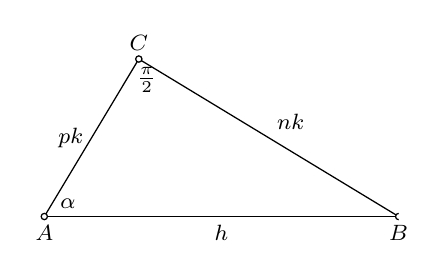
\begin{tikzpicture}
                            % \clip (0,0) rectangle (14.000000,10.000000);
                            {\footnotesize
                            
                            % Marking point C by circle
                            \draw [line width=0.016cm] (2.700000,3.500000) circle (0.040000);%
                            \draw (2.700000,3.500000) node [anchor=south] { $C$ };%
                            
                            % Marking point A by circle
                            \draw [line width=0.016cm] (1.500000,1.500000) circle (0.040000);%
                            \draw (1.500000,1.500000) node [anchor=north] { $A$ };%
                            
                            % Marking point B by circle
                            \draw [line width=0.016cm] (6.000000,1.540000) arc (90:269:0.040000 and 0.040000) -- (6.000000,1.460000);%
                            \draw (6.000000,1.500000) node [anchor=north] { $B$ };%
                            
                            % Drawing segment A C
                            \draw [line width=0.016cm] (1.520580,1.534300) -- (2.679420,3.465700);%
                            
                            % Drawing segment A B
                            \draw [line width=0.016cm] (1.540000,1.500000) -- (5.960000,1.500000);%
                            
                            % Drawing segment B C
                            \draw [line width=0.016cm] (5.965792,1.520732) -- (2.734208,3.479268);%
                            
                            % Marking point \alpha
                            \draw (1.800000,1.500000) node [anchor=south] { $\alpha$ };%
                            
                            % Marking point \frac{\pi}{2}
                            \draw (2.800000,3.500000) node [anchor=north] { $\frac{\pi}{2}$ };%
                            
                            % Marking point h
                            \draw (3.750000,1.500000) node [anchor=north] { $h$ };%
                            
                            % Marking point pk
                            \draw (2.100000,2.500000) node [anchor=east] { $pk$ };%
                            
                            % Marking point nk
                            \draw (4.350000,2.500000) node [anchor=south west] { $nk$ };%
                            }
                            \end{tikzpicture}
                        \end{figure}
                        ~\\
                        ~\\
                        \textbf{Kotangens} kota $\alpha$ je količnik med kotu $\alpha$ priležno kateto in nasprotno kateto: $$\cot\alpha = \frac{\textrm{priležna kateta}}{\textrm{nasprotna kateta}}.$$
            \end{columns}

        \end{frame}


        %%% naloge

        \begin{frame}
            \only<2->{\begin{exampleblock}{Naloga}
                V pravokotnem trikotniku sta dolžini katet $a=12~cm$ in $b=5~cm$. 
                Natančno izračunajte vrednosti kotnih funkcij kota $\beta$.
            \end{exampleblock}}


            \only<3->{\begin{exampleblock}{Naloga}
                V pravokotnem trikotniku sta dolžini katet $a=6~cm$ in $b=5~cm$. 
                Natančno izračunajte vrednosti kotnih funkcij kota $\beta$.
            \end{exampleblock}}


            \only<4->{\begin{exampleblock}{Naloga}
                V pravokotnem trikotniku je dolžina hipotenuze $c=10$ in dolžina katete $a=6$. 
                Natančno izračunajte vrednosti kotnih funkcij za kot $\alpha$.
            \end{exampleblock}}

        \end{frame}


        \begin{frame}
            \only<2->{\begin{exampleblock}{Naloga}
                Načrtajte pravokotni trikotnik $\triangle ABC$, v katerem velja:
                \begin{itemize}
                    \item $\displaystyle \sin\alpha=\dfrac{2}{5}$ \\~
                    \item $\displaystyle \cos\alpha=\dfrac{5}{6}$ \\~
                    \item $\displaystyle \tan\alpha=\dfrac{3}{7}$ \\~
                    \item $\displaystyle \cos\beta=\dfrac{4}{7}$ \\~
                    \item $\displaystyle \tan\beta=\dfrac{0.3}{0.2}$ \\~
                \end{itemize}
            \end{exampleblock}}

        \end{frame}




%%%%%%%%%%%%%%%%%%%%%%%%%%%%%%%%%%%%%%%%%%%%%%%%%%%%%%%%%%%
    \subsection{Računanje vrednosti kotnih funkcij}

        \begin{frame}
            \frametitle{Vrednosti kotnih funkcij nekaterih kotov}

            % \large\textbf{Vrednosti kotnih funkcij nekaterih kotov}
            % ~\\
            % \normalsize

            \only<2->{\begin{block}{}
                \begin{table}
                    \centering
                    \large
                    \addtolength{\tabcolsep}{6pt}
                    \renewcommand{\arraystretch}{1.5}                
                    \begin{tabular}{||c|c||c|c|c|c||} 
                        \hhline{|t:==:t:====:t|}
                        \rowcolor[rgb]{0.863,0.745,0.745}  
                                $\varphi~\left[\textrm{rad}\right] $ & $\varphi~\left[^\circ\right] $ & $\sin\varphi$ & $\cos\varphi$ & $\tan\varphi$ & $\cot\varphi$  \\ 
                        \hhline{|:==::====:|}
                                $0$ & $0$  & $0$ & $1$ & $0$ & /  \\ 
                        \hline
                                $\frac{\pi}{6}$ & $30^\circ$ & $\frac{1}{2}$ & $\frac{\sqrt{3}}{2}$ & $\frac{\sqrt{3}}{3}$ & $\sqrt{3}$  \\ 
                        \hline
                                $\frac{\pi}{4}$ & $45^\circ$ & $\frac{\sqrt{2}}{2}$ & $\frac{\sqrt{2}}{2}$ & $1$ & $1$  \\ 
                        \hline
                                $\frac{\pi}{3}$ & $60^\circ$ & $\frac{\sqrt{3}}{2}$ & $\frac{1}{2}$ & $\sqrt{3}$ & $\frac{\sqrt{3}}{3}$  \\ 
                        \hline
                                $\frac{\pi}{2}$ & $90^\circ$ & $1$ & $0$ & / & $0$  \\  
                        % \hline
                        %         $\pi$ & $180^\circ$ & $0$ & $-1$ & $0$ & /  \\ 
                        % \hline
                        %         $\frac{3\pi}{2}$ & $270^\circ$ & $-1$ & $0$ & / & $0$  \\ 
                        \hhline{|b:==:b:====:b|}
                    \end{tabular}
                \end{table}
            \end{block}}
        \end{frame}

        \begin{frame}
            \frametitle{Kotne funkcije komplementarnih kotov}

            \begin{alertblock}{}
                Sinus kota je enak kosinusu komplementarnega kota in obratno.
                $$ \sin\left({\frac{\pi}{2}-\varphi}\right) = \cos\varphi $$
                $$ \cos\left({\frac{\pi}{2}-\varphi}\right) = \sin\varphi $$
            \end{alertblock}

            \begin{alertblock}{}
                Tangens kota je enak kotangensu komplementarnega kota in obratno.
                $$ \tan\left({\frac{\pi}{2}-\varphi}\right) = \cot\varphi $$
                $$ \cot\left({\frac{\pi}{2}-\varphi}\right) = \tan\varphi $$
            \end{alertblock}
        \end{frame}


        %%%% naloge

        \begin{frame}
            \only<2->{\begin{exampleblock}{Naloga}
                Na štiri decimalna mesta natančno izračunajte vrednosti kotnih funkcij za kot $x$.
                \begin{itemize}
                    \item $x=55^\circ$
                    \item $x=39^\circ$
                    \item $x=12^\circ$
                \end{itemize}
            \end{exampleblock}}


            \only<3->{\begin{exampleblock}{Naloga}
                Na minuto natančno izračunaj velikost kota, če je:
                \begin{itemize}
                    \item $\sin{x}=0.25$
                    \item $\cos{x}=0.6$
                    \item $\tan{x}=3$
                    \item $\sin{x}=2$
                    \item $\cos{x}=\dfrac{2}{5}$
                \end{itemize}
            \end{exampleblock}}

        \end{frame}


        \begin{frame}
            \only<2->{\begin{exampleblock}{Naloga}
                Natančno izračunajte vrednost izraza.
                \begin{itemize}
                    \begin{columns}
                        \column{0.42\textwidth}
                            \item $\displaystyle \sin{90^\circ}+\cos{0^\circ}+\tan{45^\circ}$ \\~\\~
                            \item $\displaystyle \dfrac{\tan{30^\circ}}{\sin{60^\circ}}-\dfrac{\tan{60^\circ}}{\cos{60^\circ}}$ \\~\\~
                            \item $\displaystyle \tan{30^\circ}\cdot\dfrac{\sin{45^\circ}}{\cos{30^\circ}}$ \\~\\~
                            \item $\displaystyle \sin{60^\circ}+\cos{30^\circ}-\tan{45^\circ}$ \\~
                        \column{0.42\textwidth}
                            \item $\displaystyle \dfrac{\sin{30^\circ}}{\cos{30^\circ}}$ \\~\\~
                            \item $\displaystyle \dfrac{1-\sin{45^\circ}}{\cos{45^\circ}}$ \\~\\~
                            \item $\displaystyle \dfrac{\sin{90^\circ}}{1-\tan{30^\circ}}$ \\~\\~
                            \item $\displaystyle \cos{45^\circ}+\sin{45^\circ}-3\tan{30^\circ}$ \\~
                    \end{columns}
                \end{itemize}
            \end{exampleblock}}

        \end{frame}


        \begin{frame}
            \only<2->{\begin{exampleblock}{Naloga}
                V pravokotniku meri stranica $a=10~cm$, diagonala pa $14~cm$.
                Izračunajte natančno dolžino druge stranice in velikost kota med stranico $a$ in diagonalo na dve decimalki stopinje natančno.
            \end{exampleblock}}


            \only<3->{\begin{exampleblock}{Naloga}
                V enakokrakem trikotniku meri višina na osnovnico $24~cm$, osnovnica pa $14~cm$.
                Izračunajte dolžino kraka in velikost kota med krakom in osnovnico na dve decimalki stopinje natančno.
            \end{exampleblock}}


            \only<4->{\begin{exampleblock}{Naloga}
                Enakokraki trapez ima osnovnici dolgi $45~cm$ in $23~cm$, višina pa je $60~cm$.
                Izračunajte dolžino kraka in velikost kota med krakom in osnovnico na minuto natančno.
            \end{exampleblock}}

            \only<5->{\begin{exampleblock}{Naloga}
                Vrh stolpa vidimo pod kotom $19.17^\circ$, če pa se mu približamo za $50~m$, ga vidimo pod kotom $34.23^\circ$.
                Izračunajte višino stolpa, če je točka gledišča na višini $1.7~m$.
            \end{exampleblock}}


        \end{frame}


        \begin{frame}
            \only<2->{\begin{exampleblock}{Naloga}
                Koliko meri središčni kot nad lokom $AB$ v krogu s polmerom $8~cm$, če je $\lvert AB \rvert=6~cm$?
                Kot izrazite v stopinjah na štiri decimalke natančno.
            \end{exampleblock}}


            \only<3->{\begin{exampleblock}{Naloga}
                V enakokrakem trapezu z osnovnicama $12~cm$ in $6~cm$  kot ob osnovnici meri $\alpha=73^\circ$.
                Izračunajte dolžino kraka.
            \end{exampleblock}}


            \only<4->{\begin{exampleblock}{Naloga}
                Pravokotnik ima stranici dolgi $5~cm$ in $6~cm$. Na minuto natančno izračunajte kot,
                ki ga oklepata diagonali v pravokotniku.
            \end{exampleblock}}

            \only<5->{\begin{exampleblock}{Naloga}
                V rombu je dolžina diagonale $e$ dvakrat tolikšna kot dolžina diagonale $f$.
                Na minuto natančno izračunajte velikost kota $\alpha$.
            \end{exampleblock}}


        \end{frame}


%%%%%%%%%%%%%%%%%%%%%%%%%%%%%%%%%%%%%%%%%%%%%%%%%%



    \subsection{Zveze med kotnimi funkcijami}

        \begin{frame}
            \frametitle{Zveze med kotnimi funkcijami}
                           
            
        \end{frame}


        %%% naloge

        \begin{frame}
            \only<2->{\begin{exampleblock}{Naloga}
                Natančno izračunajte vrednosti preostalih kotnih funnkcj v pravokotnem trikotniku, če je kot $\alpha$ oster in velja:
                \begin{itemize}
                    \item $\cos\alpha=0.1$ \\~
                    \item $\sin\alpha=\dfrac{8}{17}$ \\~
                    \item $\tan\alpha=2$ \\~
                \end{itemize}
            \end{exampleblock}}

        \end{frame}


        \begin{frame}
            \only<2->{\begin{exampleblock}{Naloga}
                Poenostavite izraze s pomočjo zvez med kotnimi funkcijami.
                \begin{itemize}
                    \begin{columns}
                        \column{0.26\textwidth}
                            \item $\displaystyle 1-\sqrt{\left(1-\sin^2x\right)\cos^2x} $ \\~
                            \item $\displaystyle \dfrac{\sin{x}}{\tan{x}}\cdot\cos{x}-1 $ \\~
                            \item $\displaystyle \dfrac{1}{\tan{x}}+\dfrac{1-2\cos^2{x}}{\sin{x}\cos{x}} $ \\~
                        \column{0.26\textwidth}
                            \item $\displaystyle \tan^2{x}-\dfrac{1}{1-\sin^2{x}} $ \\~
                            \item $\displaystyle \cos{x}\left(1+\tan^2{x}\right) $ \\~
                            \item $\displaystyle \sin{x}+\cos^2{x}\cdot\sin^{-1}{x} $ \\~
                        \column{0.26\textwidth}
                            \item $\displaystyle \dfrac{\cos{x}}{1+\sin{x}}+\dfrac{\cos{x}}{\sin{x}-1} $ \\~
                            \item $\displaystyle \dfrac{\left(\sin{x}+\cos{x}\right)^2-1}{\tan{x}} $ \\~
                            \item $\displaystyle \dfrac{1}{\left(\dfrac{\tan^{-1}{x}\cdot\sin{x}}{\sqrt{1-\cos^2{x}}}\right)} $ \\~
                    \end{columns}
                    \begin{columns}
                        \column{0.42\textwidth}
                            \item $\displaystyle \left(\left(\tan{x}\cos{x}\right)^{-2}+\cos^{-2}{x}\right)\sin^2{x} $ \\~
                        \column{0.42\textwidth}
                            \item $\displaystyle \left(\dfrac{1}{\cot{x}}\sin^{-1}{x}\right)^{-2}+\sin{x}\tan{x}\cos{x} $ \\~
                    \end{columns}
                \end{itemize}
            \end{exampleblock}}

        \end{frame}


        \begin{frame}
            \only<2->{\begin{exampleblock}{Naloga}
                Natančno izračunajte brez uporabe računala.
                \begin{itemize}
                    \item $\displaystyle \dfrac{\cos{15^\circ}}{\sin{75^\circ}}-2\cdot\dfrac{\sin{15^\circ}}{\cos{75^\circ}}$ \\~\\~
                    \item $\displaystyle \sin^2{55^\circ}+\cos^2{45^\circ}-\dfrac{\frac{\tan{33^\circ}}{\sin{33^\circ}}}{\sin{57^\circ}}$ \\~\\~
                    \item $\displaystyle \sin^2{86^\circ}\cdot\left(\sin^2{5^\circ}+\sin^2{85^\circ}+\tan^2{4^\circ}\right)$ \\~\\~
                    \item $\displaystyle \dfrac{1-\sin^2{15^\circ}}{\sin^2{75^\circ}}$ \\~
                \end{itemize}
            \end{exampleblock}}

        \end{frame}







    \subsection{Razširitev pojma kotne funkcije do polnega kota}


        \begin{frame}
            \frametitle{Kotne funkcije v enotskem krogu}

            \begin{columns}
                \column{0.43\textwidth}
                    \begin{alertblock}{}
                        \textbf{Enotska krožnica} je krožnica s polmerom ene enote in s središčem v koordinatnem izhodišču.
                    \end{alertblock}

                    \begin{alertblock}{}
                        Kot $\varphi$ z vrhom v koordinatnem izhodišču:
                        \begin{itemize}
                            \item prvi (fiksni) krak kota leži na pozitivnem delu abscisne osi;
                            \item drugi (premični) krak določa velikost kota in leži v enem izmed štirih kvadrantov.
                        \end{itemize}
                    \end{alertblock}

                \column{0.55\textwidth}
                    \begin{figure}
                        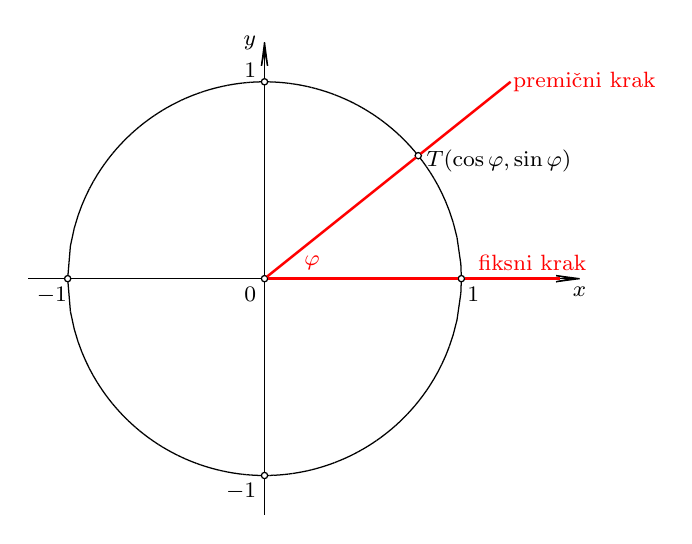
\begin{tikzpicture}
                            % \clip (0,0) rectangle (14.000000,10.000000);
                            {\footnotesize
                            
                            % Drawing 2D Cartesian system
                            \draw [line width=0.016cm] (3.000000,3.000000) circle (0.040000);%
                            \draw (3.000000,3.000000) node [anchor=north east] { $0$ };%
                            \draw [line width=0.016cm] (5.500000,3.000000) circle (0.040000);%
                            \draw (5.650000,3.000000) node [anchor=north] { $1$ };%
                            \draw [line width=0.016cm] (0.500000,3.000000) circle (0.040000);%
                            \draw (0.300000,3.000000) node [anchor=north] { $-1$ };%
                            \draw [line width=0.016cm] (3.000000,5.500000) circle (0.040000);%
                            \draw (3.000000,5.650000) node [anchor=east] { $1$ };%
                            \draw [line width=0.016cm] (3.000000,0.500000) circle (0.040000);%
                            \draw (3.000000,0.300000) node [anchor=east] { $-1$ };%
                            \draw (7.000000,3.000000) node [anchor=north] { $x$ };%
                            \draw (3.000000,6.000000) node [anchor=east] { $y$ };%
                            \draw [line width=0.016cm] (0.000000,3.000000) -- (0.460000,3.000000);%
                            \draw [line width=0.016cm] (0.540000,3.000000) -- (2.960000,3.000000);%
                            \draw [line width=0.016cm] (3.040000,3.000000) -- (5.460000,3.000000);%
                            \draw [line width=0.016cm] (5.540000,3.000000) -- (7.000000,3.000000);%
                            \draw [line width=0.016cm] (6.702567,3.039158) -- (7.000000,3.000000);%
                            \draw [line width=0.016cm] (6.702567,3.039158) -- (6.900000,3.000000);%
                            \draw [line width=0.016cm] (6.702567,2.960842) -- (7.000000,3.000000);%
                            \draw [line width=0.016cm] (6.702567,2.960842) -- (6.900000,3.000000);%
                            \draw [line width=0.016cm] (3.000000,0.000000) -- (3.000000,0.460000);%
                            \draw [line width=0.016cm] (3.000000,0.540000) -- (3.000000,2.960000);%
                            \draw [line width=0.016cm] (3.000000,3.040000) -- (3.000000,5.460000);%
                            \draw [line width=0.016cm] (3.000000,5.540000) -- (3.000000,6.000000);%
                            \draw [line width=0.016cm] (2.960842,5.702567) -- (3.000000,6.000000);%
                            \draw [line width=0.016cm] (2.960842,5.702567) -- (3.000000,5.900000);%
                            \draw [line width=0.016cm] (3.039158,5.702567) -- (3.000000,6.000000);%
                            \draw [line width=0.016cm] (3.039158,5.702567) -- (3.000000,5.900000);%
                            
                            % Drawing 2D ang conic k
                            \draw [line width=0.016cm] (0.503333,3.039861) -- (0.517361,3.207609);%
                            \draw [line width=0.016cm] (0.517361,3.207609) -- (0.534722,3.415217);%
                            \draw [line width=0.016cm] (0.503333,2.960139) -- (0.517361,2.792391);%
                            \draw [line width=0.016cm] (0.517361,2.792391) -- (0.534722,2.584783);%
                            \draw [line width=0.016cm] (0.534722,3.415217) -- (0.583333,3.640095);%
                            \draw [line width=0.016cm] (0.534722,2.584783) -- (0.583333,2.359905);%
                            \draw [line width=0.016cm] (0.583333,3.640095) -- (0.631944,3.801444);%
                            \draw [line width=0.016cm] (0.583333,2.359905) -- (0.631944,2.198556);%
                            \draw [line width=0.016cm] (0.631944,3.801444) -- (0.680556,3.932833);%
                            \draw [line width=0.016cm] (0.631944,2.198556) -- (0.680556,2.067167);%
                            \draw [line width=0.016cm] (0.680556,3.932833) -- (0.729167,4.045618);%
                            \draw [line width=0.016cm] (0.680556,2.067167) -- (0.729167,1.954382);%
                            \draw [line width=0.016cm] (0.729167,4.045618) -- (0.777778,4.145307);%
                            \draw [line width=0.016cm] (0.729167,1.954382) -- (0.777778,1.854693);%
                            \draw [line width=0.016cm] (0.777778,4.145307) -- (0.826389,4.235077);%
                            \draw [line width=0.016cm] (0.777778,1.854693) -- (0.826389,1.764923);%
                            \draw [line width=0.016cm] (0.826389,4.235077) -- (0.875000,4.316957);%
                            \draw [line width=0.016cm] (0.826389,1.764923) -- (0.875000,1.683043);%
                            \draw [line width=0.016cm] (0.875000,4.316957) -- (0.923611,4.392339);%
                            \draw [line width=0.016cm] (0.875000,1.683043) -- (0.923611,1.607661);%
                            \draw [line width=0.016cm] (0.923611,4.392339) -- (0.972222,4.462230);%
                            \draw [line width=0.016cm] (0.923611,1.607661) -- (0.972222,1.537770);%
                            \draw [line width=0.016cm] (0.972222,4.462230) -- (1.020833,4.527383);%
                            \draw [line width=0.016cm] (0.972222,1.537770) -- (1.020833,1.472617);%
                            \draw [line width=0.016cm] (1.020833,4.527383) -- (1.069444,4.588381);%
                            \draw [line width=0.016cm] (1.020833,1.472617) -- (1.069444,1.411619);%
                            \draw [line width=0.016cm] (1.069444,4.588381) -- (1.118056,4.645687);%
                            \draw [line width=0.016cm] (1.069444,1.411619) -- (1.118056,1.354313);%
                            \draw [line width=0.016cm] (1.118056,4.645687) -- (1.166667,4.699673);%
                            \draw [line width=0.016cm] (1.118056,1.354313) -- (1.166667,1.300327);%
                            \draw [line width=0.016cm] (1.166667,4.699673) -- (1.215278,4.750647);%
                            \draw [line width=0.016cm] (1.166667,1.300327) -- (1.215278,1.249353);%
                            \draw [line width=0.016cm] (1.215278,4.750647) -- (1.263889,4.798866);%
                            \draw [line width=0.016cm] (1.215278,1.249353) -- (1.263889,1.201134);%
                            \draw [line width=0.016cm] (1.263889,4.798866) -- (1.312500,4.844544);%
                            \draw [line width=0.016cm] (1.263889,1.201134) -- (1.312500,1.155456);%
                            \draw [line width=0.016cm] (1.312500,4.844544) -- (1.361111,4.887867);%
                            \draw [line width=0.016cm] (1.312500,1.155456) -- (1.361111,1.112133);%
                            \draw [line width=0.016cm] (1.361111,4.887867) -- (1.409722,4.928994);%
                            \draw [line width=0.016cm] (1.361111,1.112133) -- (1.409722,1.071006);%
                            \draw [line width=0.016cm] (1.409722,4.928994) -- (1.458333,4.968061);%
                            \draw [line width=0.016cm] (1.409722,1.071006) -- (1.458333,1.031939);%
                            \draw [line width=0.016cm] (1.458333,4.968061) -- (1.506944,5.005190);%
                            \draw [line width=0.016cm] (1.458333,1.031939) -- (1.506944,0.994810);%
                            \draw [line width=0.016cm] (1.506944,5.005190) -- (1.555556,5.040485);%
                            \draw [line width=0.016cm] (1.506944,0.994810) -- (1.555556,0.959515);%
                            \draw [line width=0.016cm] (1.555556,5.040485) -- (1.604167,5.074042);%
                            \draw [line width=0.016cm] (1.555556,0.959515) -- (1.604167,0.925958);%
                            \draw [line width=0.016cm] (1.604167,5.074042) -- (1.652778,5.105942);%
                            \draw [line width=0.016cm] (1.604167,0.925958) -- (1.652778,0.894058);%
                            \draw [line width=0.016cm] (1.652778,5.105942) -- (1.701389,5.136261);%
                            \draw [line width=0.016cm] (1.652778,0.894058) -- (1.701389,0.863739);%
                            \draw [line width=0.016cm] (1.701389,5.136261) -- (1.750000,5.165064);%
                            \draw [line width=0.016cm] (1.701389,0.863739) -- (1.750000,0.834936);%
                            \draw [line width=0.016cm] (1.750000,5.165064) -- (1.798611,5.192411);%
                            \draw [line width=0.016cm] (1.750000,0.834936) -- (1.798611,0.807589);%
                            \draw [line width=0.016cm] (1.798611,5.192411) -- (1.847222,5.218356);%
                            \draw [line width=0.016cm] (1.798611,0.807589) -- (1.847222,0.781644);%
                            \draw [line width=0.016cm] (1.847222,5.218356) -- (1.895833,5.242948);%
                            \draw [line width=0.016cm] (1.847222,0.781644) -- (1.895833,0.757052);%
                            \draw [line width=0.016cm] (1.895833,5.242948) -- (1.944444,5.266231);%
                            \draw [line width=0.016cm] (1.895833,0.757052) -- (1.944444,0.733769);%
                            \draw [line width=0.016cm] (1.944444,5.266231) -- (1.993056,5.288244);%
                            \draw [line width=0.016cm] (1.944444,0.733769) -- (1.993056,0.711756);%
                            \draw [line width=0.016cm] (1.993056,5.288244) -- (2.041667,5.309025);%
                            \draw [line width=0.016cm] (1.993056,0.711756) -- (2.041667,0.690975);%
                            \draw [line width=0.016cm] (2.041667,5.309025) -- (2.090278,5.328606);%
                            \draw [line width=0.016cm] (2.041667,0.690975) -- (2.090278,0.671394);%
                            \draw [line width=0.016cm] (2.090278,5.328606) -- (2.138889,5.347017);%
                            \draw [line width=0.016cm] (2.090278,0.671394) -- (2.138889,0.652983);%
                            \draw [line width=0.016cm] (2.138889,5.347017) -- (2.187500,5.364285);%
                            \draw [line width=0.016cm] (2.138889,0.652983) -- (2.187500,0.635715);%
                            \draw [line width=0.016cm] (2.187500,5.364285) -- (2.236111,5.380436);%
                            \draw [line width=0.016cm] (2.187500,0.635715) -- (2.236111,0.619564);%
                            \draw [line width=0.016cm] (2.236111,5.380436) -- (2.284722,5.395491);%
                            \draw [line width=0.016cm] (2.236111,0.619564) -- (2.284722,0.604509);%
                            \draw [line width=0.016cm] (2.284722,5.395491) -- (2.333333,5.409472);%
                            \draw [line width=0.016cm] (2.284722,0.604509) -- (2.333333,0.590528);%
                            \draw [line width=0.016cm] (2.333333,5.409472) -- (2.381944,5.422397);%
                            \draw [line width=0.016cm] (2.333333,0.590528) -- (2.381944,0.577603);%
                            \draw [line width=0.016cm] (2.381944,5.422397) -- (2.430556,5.434283);%
                            \draw [line width=0.016cm] (2.381944,0.577603) -- (2.430556,0.565717);%
                            \draw [line width=0.016cm] (2.430556,5.434283) -- (2.479167,5.445145);%
                            \draw [line width=0.016cm] (2.430556,0.565717) -- (2.479167,0.554855);%
                            \draw [line width=0.016cm] (2.479167,5.445145) -- (2.527778,5.454996);%
                            \draw [line width=0.016cm] (2.479167,0.554855) -- (2.527778,0.545004);%
                            \draw [line width=0.016cm] (2.527778,5.454996) -- (2.576389,5.463849);%
                            \draw [line width=0.016cm] (2.527778,0.545004) -- (2.576389,0.536151);%
                            \draw [line width=0.016cm] (2.576389,5.463849) -- (2.625000,5.471715);%
                            \draw [line width=0.016cm] (2.576389,0.536151) -- (2.625000,0.528285);%
                            \draw [line width=0.016cm] (2.625000,5.471715) -- (2.673611,5.478602);%
                            \draw [line width=0.016cm] (2.625000,0.528285) -- (2.673611,0.521398);%
                            \draw [line width=0.016cm] (2.673611,5.478602) -- (2.722222,5.484520);%
                            \draw [line width=0.016cm] (2.673611,0.521398) -- (2.722222,0.515480);%
                            \draw [line width=0.016cm] (2.722222,5.484520) -- (2.770833,5.489474);%
                            \draw [line width=0.016cm] (2.722222,0.515480) -- (2.770833,0.510526);%
                            \draw [line width=0.016cm] (2.770833,5.489474) -- (2.819444,5.493471);%
                            \draw [line width=0.016cm] (2.770833,0.510526) -- (2.819444,0.506529);%
                            \draw [line width=0.016cm] (2.819444,5.493471) -- (2.868056,5.496516);%
                            \draw [line width=0.016cm] (2.819444,0.506529) -- (2.868056,0.503484);%
                            \draw [line width=0.016cm] (2.868056,5.496516) -- (2.916667,5.498611);%
                            \draw [line width=0.016cm] (2.868056,0.503484) -- (2.916667,0.501389);%
                            \draw [line width=0.016cm] (2.916667,5.498611) -- (2.960002,5.499634);%
                            \draw [line width=0.016cm] (2.916667,0.501389) -- (2.960002,0.500366);%
                            \draw [line width=0.016cm] (3.039998,5.499562) -- (3.062500,5.499219);%
                            \draw [line width=0.016cm] (3.039998,0.500438) -- (3.062500,0.500781);%
                            \draw [line width=0.016cm] (3.062500,5.499219) -- (3.111111,5.497530);%
                            \draw [line width=0.016cm] (3.062500,0.500781) -- (3.111111,0.502470);%
                            \draw [line width=0.016cm] (3.111111,5.497530) -- (3.159722,5.494893);%
                            \draw [line width=0.016cm] (3.111111,0.502470) -- (3.159722,0.505107);%
                            \draw [line width=0.016cm] (3.159722,5.494893) -- (3.208333,5.491304);%
                            \draw [line width=0.016cm] (3.159722,0.505107) -- (3.208333,0.508696);%
                            \draw [line width=0.016cm] (3.208333,5.491304) -- (3.256944,5.486761);%
                            \draw [line width=0.016cm] (3.208333,0.508696) -- (3.256944,0.513239);%
                            \draw [line width=0.016cm] (3.256944,5.486761) -- (3.305556,5.481257);%
                            \draw [line width=0.016cm] (3.256944,0.513239) -- (3.305556,0.518743);%
                            \draw [line width=0.016cm] (3.305556,5.481257) -- (3.354167,5.474786);%
                            \draw [line width=0.016cm] (3.305556,0.518743) -- (3.354167,0.525214);%
                            \draw [line width=0.016cm] (3.354167,5.474786) -- (3.402778,5.467341);%
                            \draw [line width=0.016cm] (3.354167,0.525214) -- (3.402778,0.532659);%
                            \draw [line width=0.016cm] (3.402778,5.467341) -- (3.451389,5.458912);%
                            \draw [line width=0.016cm] (3.402778,0.532659) -- (3.451389,0.541088);%
                            \draw [line width=0.016cm] (3.451389,5.458912) -- (3.500000,5.449490);%
                            \draw [line width=0.016cm] (3.451389,0.541088) -- (3.500000,0.550510);%
                            \draw [line width=0.016cm] (3.500000,5.449490) -- (3.548611,5.439062);%
                            \draw [line width=0.016cm] (3.500000,0.550510) -- (3.548611,0.560938);%
                            \draw [line width=0.016cm] (3.548611,5.439062) -- (3.597222,5.427617);%
                            \draw [line width=0.016cm] (3.548611,0.560938) -- (3.597222,0.572383);%
                            \draw [line width=0.016cm] (3.597222,5.427617) -- (3.645833,5.415140);%
                            \draw [line width=0.016cm] (3.597222,0.572383) -- (3.645833,0.584860);%
                            \draw [line width=0.016cm] (3.645833,5.415140) -- (3.694444,5.401613);%
                            \draw [line width=0.016cm] (3.645833,0.584860) -- (3.694444,0.598387);%
                            \draw [line width=0.016cm] (3.694444,5.401613) -- (3.743056,5.387021);%
                            \draw [line width=0.016cm] (3.694444,0.598387) -- (3.743056,0.612979);%
                            \draw [line width=0.016cm] (3.743056,5.387021) -- (3.791667,5.371342);%
                            \draw [line width=0.016cm] (3.743056,0.612979) -- (3.791667,0.628658);%
                            \draw [line width=0.016cm] (3.791667,5.371342) -- (3.840278,5.354556);%
                            \draw [line width=0.016cm] (3.791667,0.628658) -- (3.840278,0.645444);%
                            \draw [line width=0.016cm] (3.840278,5.354556) -- (3.888889,5.336638);%
                            \draw [line width=0.016cm] (3.840278,0.645444) -- (3.888889,0.663362);%
                            \draw [line width=0.016cm] (3.888889,5.336638) -- (3.937500,5.317562);%
                            \draw [line width=0.016cm] (3.888889,0.663362) -- (3.937500,0.682438);%
                            \draw [line width=0.016cm] (3.937500,5.317562) -- (3.986111,5.297299);%
                            \draw [line width=0.016cm] (3.937500,0.682438) -- (3.986111,0.702701);%
                            \draw [line width=0.016cm] (3.986111,5.297299) -- (4.034722,5.275819);%
                            \draw [line width=0.016cm] (3.986111,0.702701) -- (4.034722,0.724181);%
                            \draw [line width=0.016cm] (4.034722,5.275819) -- (4.083333,5.253084);%
                            \draw [line width=0.016cm] (4.034722,0.724181) -- (4.083333,0.746916);%
                            \draw [line width=0.016cm] (4.083333,5.253084) -- (4.131944,5.229058);%
                            \draw [line width=0.016cm] (4.083333,0.746916) -- (4.131944,0.770942);%
                            \draw [line width=0.016cm] (4.131944,5.229058) -- (4.180556,5.203699);%
                            \draw [line width=0.016cm] (4.131944,0.770942) -- (4.180556,0.796301);%
                            \draw [line width=0.016cm] (4.180556,5.203699) -- (4.229167,5.176959);%
                            \draw [line width=0.016cm] (4.180556,0.796301) -- (4.229167,0.823041);%
                            \draw [line width=0.016cm] (4.229167,5.176959) -- (4.277778,5.148787);%
                            \draw [line width=0.016cm] (4.229167,0.823041) -- (4.277778,0.851213);%
                            \draw [line width=0.016cm] (4.277778,5.148787) -- (4.326389,5.119125);%
                            \draw [line width=0.016cm] (4.277778,0.851213) -- (4.326389,0.880875);%
                            \draw [line width=0.016cm] (4.326389,5.119125) -- (4.375000,5.087912);%
                            \draw [line width=0.016cm] (4.326389,0.880875) -- (4.375000,0.912088);%
                            \draw [line width=0.016cm] (4.375000,5.087912) -- (4.423611,5.055075);%
                            \draw [line width=0.016cm] (4.375000,0.912088) -- (4.423611,0.944925);%
                            \draw [line width=0.016cm] (4.423611,5.055075) -- (4.472222,5.020535);%
                            \draw [line width=0.016cm] (4.423611,0.944925) -- (4.472222,0.979465);%
                            \draw [line width=0.016cm] (4.472222,5.020535) -- (4.520833,4.984204);%
                            \draw [line width=0.016cm] (4.472222,0.979465) -- (4.520833,1.015796);%
                            \draw [line width=0.016cm] (4.520833,4.984204) -- (4.569444,4.945982);%
                            \draw [line width=0.016cm] (4.520833,1.015796) -- (4.569444,1.054018);%
                            \draw [line width=0.016cm] (4.569444,4.945982) -- (4.618056,4.905753);%
                            \draw [line width=0.016cm] (4.569444,1.054018) -- (4.618056,1.094247);%
                            \draw [line width=0.016cm] (4.618056,4.905753) -- (4.666667,4.863390);%
                            \draw [line width=0.016cm] (4.618056,1.094247) -- (4.666667,1.136610);%
                            \draw [line width=0.016cm] (4.666667,4.863390) -- (4.715278,4.818742);%
                            \draw [line width=0.016cm] (4.666667,1.136610) -- (4.715278,1.181258);%
                            \draw [line width=0.016cm] (4.715278,4.818742) -- (4.763889,4.771637);%
                            \draw [line width=0.016cm] (4.715278,1.181258) -- (4.763889,1.228363);%
                            \draw [line width=0.016cm] (4.763889,4.771637) -- (4.812500,4.721872);%
                            \draw [line width=0.016cm] (4.763889,1.228363) -- (4.812500,1.278128);%
                            \draw [line width=0.016cm] (4.812500,4.721872) -- (4.861111,4.669211);%
                            \draw [line width=0.016cm] (4.812500,1.278128) -- (4.861111,1.330789);%
                            \draw [line width=0.016cm] (4.861111,4.669211) -- (4.909722,4.613369);%
                            \draw [line width=0.016cm] (4.861111,1.330789) -- (4.909722,1.386631);%
                            \draw [line width=0.016cm] (4.909722,4.613369) -- (4.926728,4.592602);%
                            \draw [line width=0.016cm] (4.909722,1.386631) -- (4.958333,1.445995);%
                            \draw [line width=0.016cm] (4.976673,4.530120) -- (5.006944,4.490696);%
                            \draw [line width=0.016cm] (4.958333,1.445995) -- (5.006944,1.509304);%
                            \draw [line width=0.016cm] (5.006944,4.490696) -- (5.055556,4.422916);%
                            \draw [line width=0.016cm] (5.006944,1.509304) -- (5.055556,1.577084);%
                            \draw [line width=0.016cm] (5.055556,4.422916) -- (5.104167,4.349994);%
                            \draw [line width=0.016cm] (5.055556,1.577084) -- (5.104167,1.650006);%
                            \draw [line width=0.016cm] (5.104167,4.349994) -- (5.152778,4.271042);%
                            \draw [line width=0.016cm] (5.104167,1.650006) -- (5.152778,1.728958);%
                            \draw [line width=0.016cm] (5.152778,4.271042) -- (5.201389,4.184857);%
                            \draw [line width=0.016cm] (5.152778,1.728958) -- (5.201389,1.815143);%
                            \draw [line width=0.016cm] (5.201389,4.184857) -- (5.250000,4.089725);%
                            \draw [line width=0.016cm] (5.201389,1.815143) -- (5.250000,1.910275);%
                            \draw [line width=0.016cm] (5.250000,4.089725) -- (5.298611,3.983050);%
                            \draw [line width=0.016cm] (5.250000,1.910275) -- (5.298611,2.016950);%
                            \draw [line width=0.016cm] (5.298611,3.983050) -- (5.347222,3.860551);%
                            \draw [line width=0.016cm] (5.298611,2.016950) -- (5.347222,2.139449);%
                            \draw [line width=0.016cm] (5.347222,3.860551) -- (5.395833,3.714131);%
                            \draw [line width=0.016cm] (5.347222,2.139449) -- (5.395833,2.285869);%
                            \draw [line width=0.016cm] (5.395833,3.714131) -- (5.444444,3.524110);%
                            \draw [line width=0.016cm] (5.395833,2.285869) -- (5.444444,2.475890);%
                            \draw [line width=0.016cm] (5.444444,3.524110) -- (5.493056,3.186210);%
                            \draw [line width=0.016cm] (5.444444,2.475890) -- (5.493056,2.813790);%
                            \draw [line width=0.016cm] (5.498509,3.039972) -- (5.496528,3.093105);%
                            \draw [line width=0.016cm] (5.496528,3.093105) -- (5.493056,3.186210);%
                            \draw [line width=0.016cm] (5.498509,2.960028) -- (5.496528,2.906895);%
                            \draw [line width=0.016cm] (5.496528,2.906895) -- (5.493056,2.813790);%
                            
                            % Marking point T(\cos\varphi,\sin\varphi) by circle
                            \draw [line width=0.016cm] (4.952172,4.561738) circle (0.040000);%
                            \draw (4.952172,4.500000) node [anchor=west] { $T(\cos\varphi,\sin\varphi)$ };%
                            
                            % Changing color 255 0 0
                            \definecolor{r255g0b0}{rgb}{1.000000,0.000000,0.000000}%
                            \color{r255g0b0}% 
                            
                            % Marking point \textrm{fiksni~krak}
                            \draw (6.400000,3.000000) node [anchor=south] { $\textrm{fiksni~krak}$ };%
                            
                            % Marking point \textrm{premični~krak}
                            \draw (6.050000,5.500000) node [anchor=west] { $\textrm{premični~krak}$ };%

                            % Drawing segment S L
                            \draw [line width=0.032cm] (3.040000,3.000000) -- (5.460000,3.000000);%
                            \draw [line width=0.032cm] (5.540000,3.000000) -- (6.750000,3.000000);%

                            % Drawing segment S X
                            \draw [line width=0.032cm] (3.031235,3.024988) -- (4.920937,4.536750);%
                            \draw [line width=0.032cm] (4.983407,4.586725) -- (6.125000,5.500000);%

                            % Marking point \varphi
                            \draw (3.400000,3.000000) node [anchor=south west] { $\varphi$ };%
                            \color{black}
                            }
                        \end{tikzpicture}
                    \end{figure}
            \end{columns}
            ~\\
            ~\\




        \end{frame}

        \begin{frame}

            \begin{columns}
                \column{0.43\textwidth}
                    \begin{alertblock}{}
                        \textbf{Sinus} kota $\varphi$ je enak oridnati presečišča premičnega kraka z enotsko krožnico.
                    \end{alertblock}

                    \begin{alertblock}{}
                        \textbf{Kosinus} kota $\varphi$ je enak abscisi presečišča premičnega kraka z enotsko krožnico.
                    \end{alertblock}

                    \begin{alertblock}{}
                        \textbf{Tangens} kota $\varphi$ je enak ordinati presečišča premičnega kraka z navpično tangento enotskega kroga v točki $(1,0)$.
                    \end{alertblock}

                    \begin{alertblock}{}
                        \textbf{Kotangens} kota $\varphi$ je enak abscisi presečišča premičnega kraka z vodoravno tangento enotskega korga v točki $(0,1)$.
                    \end{alertblock}

                \column{0.55\textwidth}
                    \begin{figure}
                        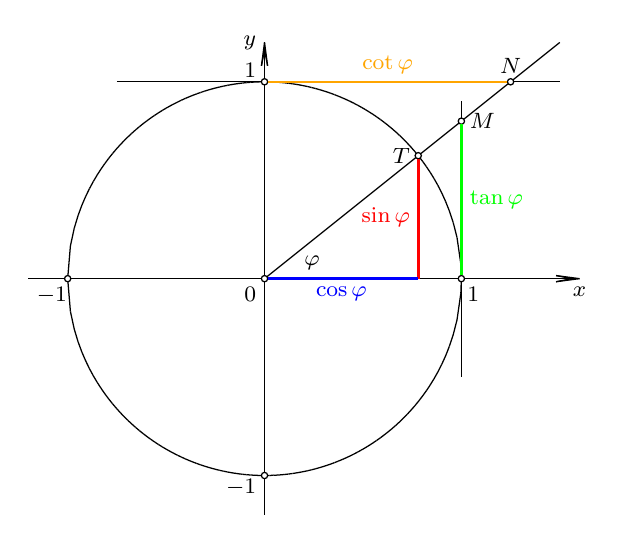
\begin{tikzpicture}
                            % \clip (0,0) rectangle (14.000000,10.000000);
                            {\footnotesize
                            
                            % Drawing 2D Cartesian system
                            \draw [line width=0.016cm] (3.000000,3.000000) circle (0.040000);%
                            \draw (3.000000,3.000000) node [anchor=north east] { $0$ };%
                            \draw [line width=0.016cm] (5.500000,3.000000) circle (0.040000);%
                            \draw (5.650000,3.000000) node [anchor=north] { $1$ };%
                            \draw [line width=0.016cm] (0.500000,3.000000) circle (0.040000);%
                            \draw (0.300000,3.000000) node [anchor=north] { $-1$ };%
                            \draw [line width=0.016cm] (3.000000,5.500000) circle (0.040000);%
                            \draw (3.000000,5.650000) node [anchor=east] { $1$ };%
                            \draw [line width=0.016cm] (3.000000,0.500000) circle (0.040000);%
                            \draw (3.000000,0.350000) node [anchor=east] { $-1$ };%
                            \draw (7.000000,3.000000) node [anchor=north] { $x$ };%
                            \draw (3.000000,6.000000) node [anchor=east] { $y$ };%
                            \draw [line width=0.016cm] (0.000000,3.000000) -- (0.460000,3.000000);%
                            \draw [line width=0.016cm] (0.540000,3.000000) -- (2.960000,3.000000);%
                            \draw [line width=0.016cm] (3.040000,3.000000) -- (5.460000,3.000000);%
                            \draw [line width=0.016cm] (5.540000,3.000000) -- (7.000000,3.000000);%
                            \draw [line width=0.016cm] (6.702567,3.039158) -- (7.000000,3.000000);%
                            \draw [line width=0.016cm] (6.702567,3.039158) -- (6.900000,3.000000);%
                            \draw [line width=0.016cm] (6.702567,2.960842) -- (7.000000,3.000000);%
                            \draw [line width=0.016cm] (6.702567,2.960842) -- (6.900000,3.000000);%
                            \draw [line width=0.016cm] (3.000000,0.000000) -- (3.000000,0.460000);%
                            \draw [line width=0.016cm] (3.000000,0.540000) -- (3.000000,2.960000);%
                            \draw [line width=0.016cm] (3.000000,3.040000) -- (3.000000,5.460000);%
                            \draw [line width=0.016cm] (3.000000,5.540000) -- (3.000000,6.000000);%
                            \draw [line width=0.016cm] (2.960842,5.702567) -- (3.000000,6.000000);%
                            \draw [line width=0.016cm] (2.960842,5.702567) -- (3.000000,5.900000);%
                            \draw [line width=0.016cm] (3.039158,5.702567) -- (3.000000,6.000000);%
                            \draw [line width=0.016cm] (3.039158,5.702567) -- (3.000000,5.900000);%
                            
                            % Drawing 2D ang conic k
                            \draw [line width=0.016cm] (0.503333,3.039861) -- (0.517361,3.207609);%
                            \draw [line width=0.016cm] (0.517361,3.207609) -- (0.534722,3.415217);%
                            \draw [line width=0.016cm] (0.503333,2.960139) -- (0.517361,2.792391);%
                            \draw [line width=0.016cm] (0.517361,2.792391) -- (0.534722,2.584783);%
                            \draw [line width=0.016cm] (0.534722,3.415217) -- (0.583333,3.640095);%
                            \draw [line width=0.016cm] (0.534722,2.584783) -- (0.583333,2.359905);%
                            \draw [line width=0.016cm] (0.583333,3.640095) -- (0.631944,3.801444);%
                            \draw [line width=0.016cm] (0.583333,2.359905) -- (0.631944,2.198556);%
                            \draw [line width=0.016cm] (0.631944,3.801444) -- (0.680556,3.932833);%
                            \draw [line width=0.016cm] (0.631944,2.198556) -- (0.680556,2.067167);%
                            \draw [line width=0.016cm] (0.680556,3.932833) -- (0.729167,4.045618);%
                            \draw [line width=0.016cm] (0.680556,2.067167) -- (0.729167,1.954382);%
                            \draw [line width=0.016cm] (0.729167,4.045618) -- (0.777778,4.145307);%
                            \draw [line width=0.016cm] (0.729167,1.954382) -- (0.777778,1.854693);%
                            \draw [line width=0.016cm] (0.777778,4.145307) -- (0.826389,4.235077);%
                            \draw [line width=0.016cm] (0.777778,1.854693) -- (0.826389,1.764923);%
                            \draw [line width=0.016cm] (0.826389,4.235077) -- (0.875000,4.316957);%
                            \draw [line width=0.016cm] (0.826389,1.764923) -- (0.875000,1.683043);%
                            \draw [line width=0.016cm] (0.875000,4.316957) -- (0.923611,4.392339);%
                            \draw [line width=0.016cm] (0.875000,1.683043) -- (0.923611,1.607661);%
                            \draw [line width=0.016cm] (0.923611,4.392339) -- (0.972222,4.462230);%
                            \draw [line width=0.016cm] (0.923611,1.607661) -- (0.972222,1.537770);%
                            \draw [line width=0.016cm] (0.972222,4.462230) -- (1.020833,4.527383);%
                            \draw [line width=0.016cm] (0.972222,1.537770) -- (1.020833,1.472617);%
                            \draw [line width=0.016cm] (1.020833,4.527383) -- (1.069444,4.588381);%
                            \draw [line width=0.016cm] (1.020833,1.472617) -- (1.069444,1.411619);%
                            \draw [line width=0.016cm] (1.069444,4.588381) -- (1.118056,4.645687);%
                            \draw [line width=0.016cm] (1.069444,1.411619) -- (1.118056,1.354313);%
                            \draw [line width=0.016cm] (1.118056,4.645687) -- (1.166667,4.699673);%
                            \draw [line width=0.016cm] (1.118056,1.354313) -- (1.166667,1.300327);%
                            \draw [line width=0.016cm] (1.166667,4.699673) -- (1.215278,4.750647);%
                            \draw [line width=0.016cm] (1.166667,1.300327) -- (1.215278,1.249353);%
                            \draw [line width=0.016cm] (1.215278,4.750647) -- (1.263889,4.798866);%
                            \draw [line width=0.016cm] (1.215278,1.249353) -- (1.263889,1.201134);%
                            \draw [line width=0.016cm] (1.263889,4.798866) -- (1.312500,4.844544);%
                            \draw [line width=0.016cm] (1.263889,1.201134) -- (1.312500,1.155456);%
                            \draw [line width=0.016cm] (1.312500,4.844544) -- (1.361111,4.887867);%
                            \draw [line width=0.016cm] (1.312500,1.155456) -- (1.361111,1.112133);%
                            \draw [line width=0.016cm] (1.361111,4.887867) -- (1.409722,4.928994);%
                            \draw [line width=0.016cm] (1.361111,1.112133) -- (1.409722,1.071006);%
                            \draw [line width=0.016cm] (1.409722,4.928994) -- (1.458333,4.968061);%
                            \draw [line width=0.016cm] (1.409722,1.071006) -- (1.458333,1.031939);%
                            \draw [line width=0.016cm] (1.458333,4.968061) -- (1.506944,5.005190);%
                            \draw [line width=0.016cm] (1.458333,1.031939) -- (1.506944,0.994810);%
                            \draw [line width=0.016cm] (1.506944,5.005190) -- (1.555556,5.040485);%
                            \draw [line width=0.016cm] (1.506944,0.994810) -- (1.555556,0.959515);%
                            \draw [line width=0.016cm] (1.555556,5.040485) -- (1.604167,5.074042);%
                            \draw [line width=0.016cm] (1.555556,0.959515) -- (1.604167,0.925958);%
                            \draw [line width=0.016cm] (1.604167,5.074042) -- (1.652778,5.105942);%
                            \draw [line width=0.016cm] (1.604167,0.925958) -- (1.652778,0.894058);%
                            \draw [line width=0.016cm] (1.652778,5.105942) -- (1.701389,5.136261);%
                            \draw [line width=0.016cm] (1.652778,0.894058) -- (1.701389,0.863739);%
                            \draw [line width=0.016cm] (1.701389,5.136261) -- (1.750000,5.165064);%
                            \draw [line width=0.016cm] (1.701389,0.863739) -- (1.750000,0.834936);%
                            \draw [line width=0.016cm] (1.750000,5.165064) -- (1.798611,5.192411);%
                            \draw [line width=0.016cm] (1.750000,0.834936) -- (1.798611,0.807589);%
                            \draw [line width=0.016cm] (1.798611,5.192411) -- (1.847222,5.218356);%
                            \draw [line width=0.016cm] (1.798611,0.807589) -- (1.847222,0.781644);%
                            \draw [line width=0.016cm] (1.847222,5.218356) -- (1.895833,5.242948);%
                            \draw [line width=0.016cm] (1.847222,0.781644) -- (1.895833,0.757052);%
                            \draw [line width=0.016cm] (1.895833,5.242948) -- (1.944444,5.266231);%
                            \draw [line width=0.016cm] (1.895833,0.757052) -- (1.944444,0.733769);%
                            \draw [line width=0.016cm] (1.944444,5.266231) -- (1.993056,5.288244);%
                            \draw [line width=0.016cm] (1.944444,0.733769) -- (1.993056,0.711756);%
                            \draw [line width=0.016cm] (1.993056,5.288244) -- (2.041667,5.309025);%
                            \draw [line width=0.016cm] (1.993056,0.711756) -- (2.041667,0.690975);%
                            \draw [line width=0.016cm] (2.041667,5.309025) -- (2.090278,5.328606);%
                            \draw [line width=0.016cm] (2.041667,0.690975) -- (2.090278,0.671394);%
                            \draw [line width=0.016cm] (2.090278,5.328606) -- (2.138889,5.347017);%
                            \draw [line width=0.016cm] (2.090278,0.671394) -- (2.138889,0.652983);%
                            \draw [line width=0.016cm] (2.138889,5.347017) -- (2.187500,5.364285);%
                            \draw [line width=0.016cm] (2.138889,0.652983) -- (2.187500,0.635715);%
                            \draw [line width=0.016cm] (2.187500,5.364285) -- (2.236111,5.380436);%
                            \draw [line width=0.016cm] (2.187500,0.635715) -- (2.236111,0.619564);%
                            \draw [line width=0.016cm] (2.236111,5.380436) -- (2.284722,5.395491);%
                            \draw [line width=0.016cm] (2.236111,0.619564) -- (2.284722,0.604509);%
                            \draw [line width=0.016cm] (2.284722,5.395491) -- (2.333333,5.409472);%
                            \draw [line width=0.016cm] (2.284722,0.604509) -- (2.333333,0.590528);%
                            \draw [line width=0.016cm] (2.333333,5.409472) -- (2.381944,5.422397);%
                            \draw [line width=0.016cm] (2.333333,0.590528) -- (2.381944,0.577603);%
                            \draw [line width=0.016cm] (2.381944,5.422397) -- (2.430556,5.434283);%
                            \draw [line width=0.016cm] (2.381944,0.577603) -- (2.430556,0.565717);%
                            \draw [line width=0.016cm] (2.430556,5.434283) -- (2.479167,5.445145);%
                            \draw [line width=0.016cm] (2.430556,0.565717) -- (2.479167,0.554855);%
                            \draw [line width=0.016cm] (2.479167,5.445145) -- (2.527778,5.454996);%
                            \draw [line width=0.016cm] (2.479167,0.554855) -- (2.527778,0.545004);%
                            \draw [line width=0.016cm] (2.527778,5.454996) -- (2.576389,5.463849);%
                            \draw [line width=0.016cm] (2.527778,0.545004) -- (2.576389,0.536151);%
                            \draw [line width=0.016cm] (2.576389,5.463849) -- (2.625000,5.471715);%
                            \draw [line width=0.016cm] (2.576389,0.536151) -- (2.625000,0.528285);%
                            \draw [line width=0.016cm] (2.625000,5.471715) -- (2.673611,5.478602);%
                            \draw [line width=0.016cm] (2.625000,0.528285) -- (2.673611,0.521398);%
                            \draw [line width=0.016cm] (2.673611,5.478602) -- (2.722222,5.484520);%
                            \draw [line width=0.016cm] (2.673611,0.521398) -- (2.722222,0.515480);%
                            \draw [line width=0.016cm] (2.722222,5.484520) -- (2.770833,5.489474);%
                            \draw [line width=0.016cm] (2.722222,0.515480) -- (2.770833,0.510526);%
                            \draw [line width=0.016cm] (2.770833,5.489474) -- (2.819444,5.493471);%
                            \draw [line width=0.016cm] (2.770833,0.510526) -- (2.819444,0.506529);%
                            \draw [line width=0.016cm] (2.819444,5.493471) -- (2.868056,5.496516);%
                            \draw [line width=0.016cm] (2.819444,0.506529) -- (2.868056,0.503484);%
                            \draw [line width=0.016cm] (2.868056,5.496516) -- (2.916667,5.498611);%
                            \draw [line width=0.016cm] (2.868056,0.503484) -- (2.916667,0.501389);%
                            \draw [line width=0.016cm] (2.916667,5.498611) -- (2.960002,5.499634);%
                            \draw [line width=0.016cm] (2.916667,0.501389) -- (2.960002,0.500366);%
                            \draw [line width=0.016cm] (3.039998,5.499562) -- (3.062500,5.499219);%
                            \draw [line width=0.016cm] (3.039998,0.500438) -- (3.062500,0.500781);%
                            \draw [line width=0.016cm] (3.062500,5.499219) -- (3.111111,5.497530);%
                            \draw [line width=0.016cm] (3.062500,0.500781) -- (3.111111,0.502470);%
                            \draw [line width=0.016cm] (3.111111,5.497530) -- (3.159722,5.494893);%
                            \draw [line width=0.016cm] (3.111111,0.502470) -- (3.159722,0.505107);%
                            \draw [line width=0.016cm] (3.159722,5.494893) -- (3.208333,5.491304);%
                            \draw [line width=0.016cm] (3.159722,0.505107) -- (3.208333,0.508696);%
                            \draw [line width=0.016cm] (3.208333,5.491304) -- (3.256944,5.486761);%
                            \draw [line width=0.016cm] (3.208333,0.508696) -- (3.256944,0.513239);%
                            \draw [line width=0.016cm] (3.256944,5.486761) -- (3.305556,5.481257);%
                            \draw [line width=0.016cm] (3.256944,0.513239) -- (3.305556,0.518743);%
                            \draw [line width=0.016cm] (3.305556,5.481257) -- (3.354167,5.474786);%
                            \draw [line width=0.016cm] (3.305556,0.518743) -- (3.354167,0.525214);%
                            \draw [line width=0.016cm] (3.354167,5.474786) -- (3.402778,5.467341);%
                            \draw [line width=0.016cm] (3.354167,0.525214) -- (3.402778,0.532659);%
                            \draw [line width=0.016cm] (3.402778,5.467341) -- (3.451389,5.458912);%
                            \draw [line width=0.016cm] (3.402778,0.532659) -- (3.451389,0.541088);%
                            \draw [line width=0.016cm] (3.451389,5.458912) -- (3.500000,5.449490);%
                            \draw [line width=0.016cm] (3.451389,0.541088) -- (3.500000,0.550510);%
                            \draw [line width=0.016cm] (3.500000,5.449490) -- (3.548611,5.439062);%
                            \draw [line width=0.016cm] (3.500000,0.550510) -- (3.548611,0.560938);%
                            \draw [line width=0.016cm] (3.548611,5.439062) -- (3.597222,5.427617);%
                            \draw [line width=0.016cm] (3.548611,0.560938) -- (3.597222,0.572383);%
                            \draw [line width=0.016cm] (3.597222,5.427617) -- (3.645833,5.415140);%
                            \draw [line width=0.016cm] (3.597222,0.572383) -- (3.645833,0.584860);%
                            \draw [line width=0.016cm] (3.645833,5.415140) -- (3.694444,5.401613);%
                            \draw [line width=0.016cm] (3.645833,0.584860) -- (3.694444,0.598387);%
                            \draw [line width=0.016cm] (3.694444,5.401613) -- (3.743056,5.387021);%
                            \draw [line width=0.016cm] (3.694444,0.598387) -- (3.743056,0.612979);%
                            \draw [line width=0.016cm] (3.743056,5.387021) -- (3.791667,5.371342);%
                            \draw [line width=0.016cm] (3.743056,0.612979) -- (3.791667,0.628658);%
                            \draw [line width=0.016cm] (3.791667,5.371342) -- (3.840278,5.354556);%
                            \draw [line width=0.016cm] (3.791667,0.628658) -- (3.840278,0.645444);%
                            \draw [line width=0.016cm] (3.840278,5.354556) -- (3.888889,5.336638);%
                            \draw [line width=0.016cm] (3.840278,0.645444) -- (3.888889,0.663362);%
                            \draw [line width=0.016cm] (3.888889,5.336638) -- (3.937500,5.317562);%
                            \draw [line width=0.016cm] (3.888889,0.663362) -- (3.937500,0.682438);%
                            \draw [line width=0.016cm] (3.937500,5.317562) -- (3.986111,5.297299);%
                            \draw [line width=0.016cm] (3.937500,0.682438) -- (3.986111,0.702701);%
                            \draw [line width=0.016cm] (3.986111,5.297299) -- (4.034722,5.275819);%
                            \draw [line width=0.016cm] (3.986111,0.702701) -- (4.034722,0.724181);%
                            \draw [line width=0.016cm] (4.034722,5.275819) -- (4.083333,5.253084);%
                            \draw [line width=0.016cm] (4.034722,0.724181) -- (4.083333,0.746916);%
                            \draw [line width=0.016cm] (4.083333,5.253084) -- (4.131944,5.229058);%
                            \draw [line width=0.016cm] (4.083333,0.746916) -- (4.131944,0.770942);%
                            \draw [line width=0.016cm] (4.131944,5.229058) -- (4.180556,5.203699);%
                            \draw [line width=0.016cm] (4.131944,0.770942) -- (4.180556,0.796301);%
                            \draw [line width=0.016cm] (4.180556,5.203699) -- (4.229167,5.176959);%
                            \draw [line width=0.016cm] (4.180556,0.796301) -- (4.229167,0.823041);%
                            \draw [line width=0.016cm] (4.229167,5.176959) -- (4.277778,5.148787);%
                            \draw [line width=0.016cm] (4.229167,0.823041) -- (4.277778,0.851213);%
                            \draw [line width=0.016cm] (4.277778,5.148787) -- (4.326389,5.119125);%
                            \draw [line width=0.016cm] (4.277778,0.851213) -- (4.326389,0.880875);%
                            \draw [line width=0.016cm] (4.326389,5.119125) -- (4.375000,5.087912);%
                            \draw [line width=0.016cm] (4.326389,0.880875) -- (4.375000,0.912088);%
                            \draw [line width=0.016cm] (4.375000,5.087912) -- (4.423611,5.055075);%
                            \draw [line width=0.016cm] (4.375000,0.912088) -- (4.423611,0.944925);%
                            \draw [line width=0.016cm] (4.423611,5.055075) -- (4.472222,5.020535);%
                            \draw [line width=0.016cm] (4.423611,0.944925) -- (4.472222,0.979465);%
                            \draw [line width=0.016cm] (4.472222,5.020535) -- (4.520833,4.984204);%
                            \draw [line width=0.016cm] (4.472222,0.979465) -- (4.520833,1.015796);%
                            \draw [line width=0.016cm] (4.520833,4.984204) -- (4.569444,4.945982);%
                            \draw [line width=0.016cm] (4.520833,1.015796) -- (4.569444,1.054018);%
                            \draw [line width=0.016cm] (4.569444,4.945982) -- (4.618056,4.905753);%
                            \draw [line width=0.016cm] (4.569444,1.054018) -- (4.618056,1.094247);%
                            \draw [line width=0.016cm] (4.618056,4.905753) -- (4.666667,4.863390);%
                            \draw [line width=0.016cm] (4.618056,1.094247) -- (4.666667,1.136610);%
                            \draw [line width=0.016cm] (4.666667,4.863390) -- (4.715278,4.818742);%
                            \draw [line width=0.016cm] (4.666667,1.136610) -- (4.715278,1.181258);%
                            \draw [line width=0.016cm] (4.715278,4.818742) -- (4.763889,4.771637);%
                            \draw [line width=0.016cm] (4.715278,1.181258) -- (4.763889,1.228363);%
                            \draw [line width=0.016cm] (4.763889,4.771637) -- (4.812500,4.721872);%
                            \draw [line width=0.016cm] (4.763889,1.228363) -- (4.812500,1.278128);%
                            \draw [line width=0.016cm] (4.812500,4.721872) -- (4.861111,4.669211);%
                            \draw [line width=0.016cm] (4.812500,1.278128) -- (4.861111,1.330789);%
                            \draw [line width=0.016cm] (4.861111,4.669211) -- (4.909722,4.613369);%
                            \draw [line width=0.016cm] (4.861111,1.330789) -- (4.909722,1.386631);%
                            \draw [line width=0.016cm] (4.909722,4.613369) -- (4.926728,4.592602);%
                            \draw [line width=0.016cm] (4.909722,1.386631) -- (4.958333,1.445995);%
                            \draw [line width=0.016cm] (4.976673,4.530120) -- (5.006944,4.490696);%
                            \draw [line width=0.016cm] (4.958333,1.445995) -- (5.006944,1.509304);%
                            \draw [line width=0.016cm] (5.006944,4.490696) -- (5.055556,4.422916);%
                            \draw [line width=0.016cm] (5.006944,1.509304) -- (5.055556,1.577084);%
                            \draw [line width=0.016cm] (5.055556,4.422916) -- (5.104167,4.349994);%
                            \draw [line width=0.016cm] (5.055556,1.577084) -- (5.104167,1.650006);%
                            \draw [line width=0.016cm] (5.104167,4.349994) -- (5.152778,4.271042);%
                            \draw [line width=0.016cm] (5.104167,1.650006) -- (5.152778,1.728958);%
                            \draw [line width=0.016cm] (5.152778,4.271042) -- (5.201389,4.184857);%
                            \draw [line width=0.016cm] (5.152778,1.728958) -- (5.201389,1.815143);%
                            \draw [line width=0.016cm] (5.201389,4.184857) -- (5.250000,4.089725);%
                            \draw [line width=0.016cm] (5.201389,1.815143) -- (5.250000,1.910275);%
                            \draw [line width=0.016cm] (5.250000,4.089725) -- (5.298611,3.983050);%
                            \draw [line width=0.016cm] (5.250000,1.910275) -- (5.298611,2.016950);%
                            \draw [line width=0.016cm] (5.298611,3.983050) -- (5.347222,3.860551);%
                            \draw [line width=0.016cm] (5.298611,2.016950) -- (5.347222,2.139449);%
                            \draw [line width=0.016cm] (5.347222,3.860551) -- (5.395833,3.714131);%
                            \draw [line width=0.016cm] (5.347222,2.139449) -- (5.395833,2.285869);%
                            \draw [line width=0.016cm] (5.395833,3.714131) -- (5.444444,3.524110);%
                            \draw [line width=0.016cm] (5.395833,2.285869) -- (5.444444,2.475890);%
                            \draw [line width=0.016cm] (5.444444,3.524110) -- (5.493056,3.186210);%
                            \draw [line width=0.016cm] (5.444444,2.475890) -- (5.493056,2.813790);%
                            \draw [line width=0.016cm] (5.498509,3.039972) -- (5.496528,3.093105);%
                            \draw [line width=0.016cm] (5.496528,3.093105) -- (5.493056,3.186210);%
                            \draw [line width=0.016cm] (5.498509,2.960028) -- (5.496528,2.906895);%
                            \draw [line width=0.016cm] (5.496528,2.906895) -- (5.493056,2.813790);%
                            
                            % Marking point T by circle
                            \draw [line width=0.016cm] (4.952172,4.561738) circle (0.040000);%
                            \draw (4.952172,4.561738) node [anchor=east] { $T$ };%
                            
                            % Drawing segment S X
                            \draw [line width=0.016cm] (3.031235,3.024988) -- (4.920937,4.536750);%
                            \draw [line width=0.016cm] (4.983407,4.586725) -- (5.468765,4.975012);%
                            \draw [line width=0.016cm] (5.531235,5.024988) -- (6.093765,5.475012);%
                            \draw [line width=0.016cm] (6.156235,5.524988) -- (6.750000,6.000000);%
                            
                            % Marking point \varphi
                            \draw (3.400000,3.000000) node [anchor=south west] { $\varphi$ };%
                            
                            % Marking point N by circle
                            \draw [line width=0.016cm] (6.125000,5.500000) circle (0.040000);%
                            \draw (6.125000,5.500000) node [anchor=south] { $N$ };%
                            
                            % Marking point M by circle
                            \draw [line width=0.016cm] (5.500000,5.000000) circle (0.040000);%
                            \draw (5.500000,5.000000) node [anchor=west] { $M$ };%
                            
                            % Drawing segment P E
                            \draw [line width=0.016cm] (1.125000,5.500000) -- (2.960000,5.500000);%
                            \draw [line width=0.016cm] (3.040000,5.500000) -- (6.085000,5.500000);%
                            \draw [line width=0.016cm] (6.165000,5.500000) -- (6.750000,5.500000);%
                            
                            % Drawing segment F H
                            \draw [line width=0.016cm] (5.500000,5.250000) -- (5.500000,5.040000);%
                            \draw [line width=0.016cm] (5.500000,4.960000) -- (5.500000,3.040000);%
                            \draw [line width=0.016cm] (5.500000,2.960000) -- (5.500000,1.750000);%
                            
                            % Changing color 255 0 0
                            \definecolor{r255g0b0}{rgb}{1.000000,0.000000,0.000000}%
                            \color{r255g0b0}% 
                            
                            % Marking point \sin\varphi
                            \draw (4.952172,3.780869) node [anchor=east] { $\sin\varphi$ };%
                            
                            % Drawing segment U T
                            \draw [line width=0.032cm] (4.952172,3.000000) -- (4.952172,4.521738);%
                            
                            % Changing color 0 0 255
                            \definecolor{r0g0b255}{rgb}{0.000000,0.000000,1.000000}%
                            \color{r0g0b255}% 
                            
                            % Marking point \cos\varphi
                            \draw (3.976086,3.000000) node [anchor=north] { $\cos\varphi$ };%
                            
                            % Drawing segment S U
                            \draw [line width=0.032cm] (3.040000,3.000000) -- (4.952172,3.000000);%
                            
                            % Changing color 0 255 0
                            \definecolor{r0g255b0}{rgb}{0.000000,1.000000,0.000000}%
                            \color{r0g255b0}% 
                            
                            % Marking point \tan\varphi
                            \draw (5.500000,4.000000) node [anchor=west] { $\tan\varphi$ };%
                            
                            % Drawing segment R M
                            \draw [line width=0.032cm] (5.500000,3.040000) -- (5.500000,4.960000);%
                            
                            % Changing color 255 165 0
                            \definecolor{r255g165b0}{rgb}{1.000000,0.647059,0.000000}%
                            \color{r255g165b0}% 
                            
                            % Marking point \cot\varphi
                            \draw (4.562500,5.500000) node [anchor=south] { $\cot\varphi$ };%
                            
                            % Drawing segment RR N
                            \draw [line width=0.032cm] (3.040000,5.500000) -- (6.085000,5.500000);%
                            \color{black}
                            }
                        \end{tikzpicture}                    
                    \end{figure}
            \end{columns}

        \end{frame}


        
        \begin{frame}
            \frametitle{Stopinje in radiani}

            \begin{alertblock}{Radian}
                Loku na krožnici, ki je enako dolg kot polmer krožnice, pripada središčni kot, velik $1 \ \textrm{radian}$.
                $$ 1 \ \textrm{rad}=\frac{180^\circ}{\pi}\doteq 57,3^\circ$$
            \end{alertblock}

            \begin{exampleblock}{Pretvorba med stopinjami in radiani}
                Naj bo $\varphi$ kot podan v radianih, $\phi$ pa njemu pripadajoči kot podan v stopinjah. Potem velja:
                $$ \varphi = \frac{\pi}{180^\circ}\phi$$
                in 
                $$ \phi = \frac{180^\circ}{\pi} \varphi.$$
            \end{exampleblock}
        \end{frame}



        \begin{frame}
            \frametitle{Vrednosti kotnih funkcij nekaterih kotov}

            % \large\textbf{Vrednosti kotnih funkcij nekaterih kotov}
            % ~\\
            % \normalsize

            \begin{table}
                \centering
                \large
                \addtolength{\tabcolsep}{6pt}
                \renewcommand{\arraystretch}{1.5}                
                \begin{tabular}{||c|c||c|c|c|c||} 
                    \hhline{|t:==:t:====:t|}
                    \rowcolor[rgb]{0.863,0.745,0.745}  
                            $\varphi~\left[\textrm{rad}\right] $ & $\varphi~\left[^\circ\right] $ & $\sin\varphi$ & $\cos\varphi$ & $\tan\varphi$ & $\cot\varphi$  \\ 
                    \hhline{|:==::====:|}
                            $0$ & $0$  & $0$ & $1$ & $0$ & /  \\ 
                    \hline
                            $\frac{\pi}{6}$ & $30^\circ$ & $\frac{1}{2}$ & $\frac{\sqrt{3}}{2}$ & $\frac{\sqrt{3}}{3}$ & $\sqrt{3}$  \\ 
                    \hline
                            $\frac{\pi}{4}$ & $45^\circ$ & $\frac{\sqrt{2}}{2}$ & $\frac{\sqrt{2}}{2}$ & $1$ & $1$  \\ 
                    \hline
                            $\frac{\pi}{3}$ & $60^\circ$ & $\frac{\sqrt{3}}{2}$ & $\frac{1}{2}$ & $\sqrt{3}$ & $\frac{\sqrt{3}}{3}$  \\ 
                    \hline
                            $\frac{\pi}{2}$ & $90^\circ$ & $1$ & $0$ & / & $0$  \\  
                    \hline
                            $\pi$ & $180^\circ$ & $0$ & $-1$ & $0$ & /  \\ 
                    \hline
                            $\frac{3\pi}{2}$ & $270^\circ$ & $-1$ & $0$ & / & $0$  \\ 
                    \hhline{|b:==:b:====:b|}
                \end{tabular}
            \end{table}

        \end{frame}

        \begin{frame}
            \large\textbf{Kot med $\frac{\pi}{2}$ in $\pi$}
            ~\\
            \normalsize


            \begin{columns}
                \column{0.55\textwidth}
                    \begin{figure}
                        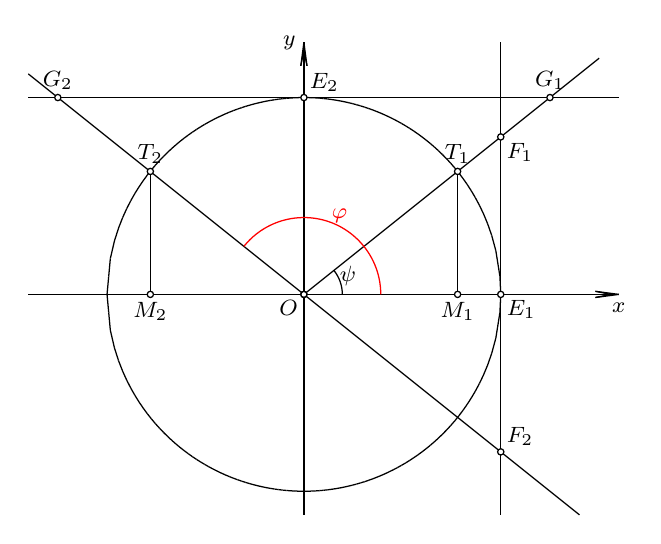
\begin{tikzpicture}
                            % \clip (0,0) rectangle (14.000000,10.000000);
                            {\footnotesize
                            
                            % Drawing 2D Cartesian system
                            \draw [line width=0.016cm] (4.000000,4.000000) circle (0.040000);%
                            % \draw (4.000000,4.000000) node [anchor=north east] { $0$ };%
                            \draw (8.000000,4.000000) node [anchor=north] { $x$ };%
                            \draw (4.000000,7.200000) node [anchor=east] { $y$ };%
                            \draw [line width=0.016cm] (0.500000,4.000000) -- (2.010000,4.000000);%
                            \draw [line width=0.016cm] (2.090000,4.000000) -- (3.960000,4.000000);%
                            \draw [line width=0.016cm] (4.040000,4.000000) -- (5.912172,4.000000);%
                            \draw [line width=0.016cm] (5.992172,4.000000) -- (6.460000,4.000000);%
                            \draw [line width=0.016cm] (6.540000,4.000000) -- (8.000000,4.000000);%
                            \draw [line width=0.016cm] (7.702567,4.039158) -- (8.000000,4.000000);%
                            \draw [line width=0.016cm] (7.702567,4.039158) -- (7.900000,4.000000);%
                            \draw [line width=0.016cm] (7.702567,3.960842) -- (8.000000,4.000000);%
                            \draw [line width=0.016cm] (7.702567,3.960842) -- (7.900000,4.000000);%
                            \draw [line width=0.016cm] (4.000000,1.200000) -- (4.000000,3.960000);%
                            \draw [line width=0.016cm] (4.000000,4.040000) -- (4.000000,6.460000);%
                            \draw [line width=0.016cm] (4.000000,6.540000) -- (4.000000,7.200000);%
                            \draw [line width=0.016cm] (3.960842,6.902567) -- (4.000000,7.200000);%
                            \draw [line width=0.016cm] (3.960842,6.902567) -- (4.000000,7.100000);%
                            \draw [line width=0.016cm] (4.039158,6.902567) -- (4.000000,7.200000);%
                            \draw [line width=0.016cm] (4.039158,6.902567) -- (4.000000,7.100000);%
                            
                            % Drawing 2D ang conic k
                            \draw [line width=0.016cm] (1.500000,4.000000) -- (1.520833,4.227265);%
                            \draw [line width=0.016cm] (1.520833,4.227265) -- (1.541667,4.454530);%
                            \draw [line width=0.016cm] (1.500000,4.000000) -- (1.520833,3.772735);%
                            \draw [line width=0.016cm] (1.520833,3.772735) -- (1.541667,3.545470);%
                            \draw [line width=0.016cm] (1.541667,4.454530) -- (1.593750,4.678204);%
                            \draw [line width=0.016cm] (1.541667,3.545470) -- (1.593750,3.321796);%
                            \draw [line width=0.016cm] (1.593750,4.678204) -- (1.645833,4.841368);%
                            \draw [line width=0.016cm] (1.593750,3.321796) -- (1.645833,3.158632);%
                            \draw [line width=0.016cm] (1.645833,4.841368) -- (1.697917,4.974891);%
                            \draw [line width=0.016cm] (1.645833,3.158632) -- (1.697917,3.025109);%
                            \draw [line width=0.016cm] (1.697917,4.974891) -- (1.750000,5.089725);%
                            \draw [line width=0.016cm] (1.697917,3.025109) -- (1.750000,2.910275);%
                            \draw [line width=0.016cm] (1.750000,5.089725) -- (1.802083,5.191286);%
                            \draw [line width=0.016cm] (1.750000,2.910275) -- (1.802083,2.808714);%
                            \draw [line width=0.016cm] (1.802083,5.191286) -- (1.854167,5.282731);%
                            \draw [line width=0.016cm] (1.802083,2.808714) -- (1.854167,2.717269);%
                            \draw [line width=0.016cm] (1.854167,5.282731) -- (1.906250,5.366093);%
                            \draw [line width=0.016cm] (1.854167,2.717269) -- (1.906250,2.633907);%
                            \draw [line width=0.016cm] (1.906250,5.366093) -- (1.958333,5.442774);%
                            \draw [line width=0.016cm] (1.906250,2.633907) -- (1.958333,2.557226);%
                            \draw [line width=0.016cm] (1.958333,5.442774) -- (2.010417,5.513789);%
                            \draw [line width=0.016cm] (1.958333,2.557226) -- (2.010417,2.486211);%
                            \draw [line width=0.016cm] (2.010417,5.513789) -- (2.024145,5.531216);%
                            \draw [line width=0.016cm] (2.010417,2.486211) -- (2.062500,2.420097);%
                            \draw [line width=0.016cm] (2.074097,5.593665) -- (2.114583,5.641708);%
                            \draw [line width=0.016cm] (2.062500,2.420097) -- (2.114583,2.358292);%
                            \draw [line width=0.016cm] (2.114583,5.641708) -- (2.166667,5.699673);%
                            \draw [line width=0.016cm] (2.114583,2.358292) -- (2.166667,2.300327);%
                            \draw [line width=0.016cm] (2.166667,5.699673) -- (2.218750,5.754180);%
                            \draw [line width=0.016cm] (2.166667,2.300327) -- (2.218750,2.245820);%
                            \draw [line width=0.016cm] (2.218750,5.754180) -- (2.270833,5.805542);%
                            \draw [line width=0.016cm] (2.218750,2.245820) -- (2.270833,2.194458);%
                            \draw [line width=0.016cm] (2.270833,5.805542) -- (2.322917,5.854020);%
                            \draw [line width=0.016cm] (2.270833,2.194458) -- (2.322917,2.145980);%
                            \draw [line width=0.016cm] (2.322917,5.854020) -- (2.375000,5.899836);%
                            \draw [line width=0.016cm] (2.322917,2.145980) -- (2.375000,2.100164);%
                            \draw [line width=0.016cm] (2.375000,5.899836) -- (2.427083,5.943176);%
                            \draw [line width=0.016cm] (2.375000,2.100164) -- (2.427083,2.056824);%
                            \draw [line width=0.016cm] (2.427083,5.943176) -- (2.479167,5.984204);%
                            \draw [line width=0.016cm] (2.427083,2.056824) -- (2.479167,2.015796);%
                            \draw [line width=0.016cm] (2.479167,5.984204) -- (2.531250,6.023060);%
                            \draw [line width=0.016cm] (2.479167,2.015796) -- (2.531250,1.976940);%
                            \draw [line width=0.016cm] (2.531250,6.023060) -- (2.583333,6.059868);%
                            \draw [line width=0.016cm] (2.531250,1.976940) -- (2.583333,1.940132);%
                            \draw [line width=0.016cm] (2.583333,6.059868) -- (2.635417,6.094734);%
                            \draw [line width=0.016cm] (2.583333,1.940132) -- (2.635417,1.905266);%
                            \draw [line width=0.016cm] (2.635417,6.094734) -- (2.687500,6.127756);%
                            \draw [line width=0.016cm] (2.635417,1.905266) -- (2.687500,1.872244);%
                            \draw [line width=0.016cm] (2.687500,6.127756) -- (2.739583,6.159016);%
                            \draw [line width=0.016cm] (2.687500,1.872244) -- (2.739583,1.840984);%
                            \draw [line width=0.016cm] (2.739583,6.159016) -- (2.791667,6.188591);%
                            \draw [line width=0.016cm] (2.739583,1.840984) -- (2.791667,1.811409);%
                            \draw [line width=0.016cm] (2.791667,6.188591) -- (2.843750,6.216548);%
                            \draw [line width=0.016cm] (2.791667,1.811409) -- (2.843750,1.783452);%
                            \draw [line width=0.016cm] (2.843750,6.216548) -- (2.895833,6.242948);%
                            \draw [line width=0.016cm] (2.843750,1.783452) -- (2.895833,1.757052);%
                            \draw [line width=0.016cm] (2.895833,6.242948) -- (2.947917,6.267845);%
                            \draw [line width=0.016cm] (2.895833,1.757052) -- (2.947917,1.732155);%
                            \draw [line width=0.016cm] (2.947917,6.267845) -- (3.000000,6.291288);%
                            \draw [line width=0.016cm] (2.947917,1.732155) -- (3.000000,1.708712);%
                            \draw [line width=0.016cm] (3.000000,6.291288) -- (3.052083,6.313321);%
                            \draw [line width=0.016cm] (3.000000,1.708712) -- (3.052083,1.686679);%
                            \draw [line width=0.016cm] (3.052083,6.313321) -- (3.104167,6.333984);%
                            \draw [line width=0.016cm] (3.052083,1.686679) -- (3.104167,1.666016);%
                            \draw [line width=0.016cm] (3.104167,6.333984) -- (3.156250,6.353314);%
                            \draw [line width=0.016cm] (3.104167,1.666016) -- (3.156250,1.646686);%
                            \draw [line width=0.016cm] (3.156250,6.353314) -- (3.208333,6.371342);%
                            \draw [line width=0.016cm] (3.156250,1.646686) -- (3.208333,1.628658);%
                            \draw [line width=0.016cm] (3.208333,6.371342) -- (3.260417,6.388099);%
                            \draw [line width=0.016cm] (3.208333,1.628658) -- (3.260417,1.611901);%
                            \draw [line width=0.016cm] (3.260417,6.388099) -- (3.312500,6.403611);%
                            \draw [line width=0.016cm] (3.260417,1.611901) -- (3.312500,1.596389);%
                            \draw [line width=0.016cm] (3.312500,6.403611) -- (3.364583,6.417901);%
                            \draw [line width=0.016cm] (3.312500,1.596389) -- (3.364583,1.582099);%
                            \draw [line width=0.016cm] (3.364583,6.417901) -- (3.416667,6.430992);%
                            \draw [line width=0.016cm] (3.364583,1.582099) -- (3.416667,1.569008);%
                            \draw [line width=0.016cm] (3.416667,6.430992) -- (3.468750,6.442903);%
                            \draw [line width=0.016cm] (3.416667,1.569008) -- (3.468750,1.557097);%
                            \draw [line width=0.016cm] (3.468750,6.442903) -- (3.520833,6.453650);%
                            \draw [line width=0.016cm] (3.468750,1.557097) -- (3.520833,1.546350);%
                            \draw [line width=0.016cm] (3.520833,6.453650) -- (3.572917,6.463250);%
                            \draw [line width=0.016cm] (3.520833,1.546350) -- (3.572917,1.536750);%
                            \draw [line width=0.016cm] (3.572917,6.463250) -- (3.625000,6.471715);%
                            \draw [line width=0.016cm] (3.572917,1.536750) -- (3.625000,1.528285);%
                            \draw [line width=0.016cm] (3.625000,6.471715) -- (3.677083,6.479057);%
                            \draw [line width=0.016cm] (3.625000,1.528285) -- (3.677083,1.520943);%
                            \draw [line width=0.016cm] (3.677083,6.479057) -- (3.729167,6.485287);%
                            \draw [line width=0.016cm] (3.677083,1.520943) -- (3.729167,1.514713);%
                            \draw [line width=0.016cm] (3.729167,6.485287) -- (3.781250,6.490411);%
                            \draw [line width=0.016cm] (3.729167,1.514713) -- (3.781250,1.509589);%
                            \draw [line width=0.016cm] (3.781250,6.490411) -- (3.833333,6.494438);%
                            \draw [line width=0.016cm] (3.781250,1.509589) -- (3.833333,1.505562);%
                            \draw [line width=0.016cm] (3.833333,6.494438) -- (3.885417,6.497373);%
                            \draw [line width=0.016cm] (3.833333,1.505562) -- (3.885417,1.502627);%
                            \draw [line width=0.016cm] (3.885417,6.497373) -- (3.937500,6.499219);%
                            \draw [line width=0.016cm] (3.885417,1.502627) -- (3.937500,1.500781);%
                            \draw [line width=0.016cm] (3.937500,6.499219) -- (3.960003,6.499547);%
                            \draw [line width=0.016cm] (3.937500,1.500781) -- (3.989583,1.500022);%
                            \draw [line width=0.016cm] (4.039999,6.499663) -- (4.041667,6.499653);%
                            \draw [line width=0.016cm] (3.989583,1.500022) -- (4.041667,1.500347);%
                            \draw [line width=0.016cm] (4.041667,6.499653) -- (4.093750,6.498242);%
                            \draw [line width=0.016cm] (4.041667,1.500347) -- (4.093750,1.501758);%
                            \draw [line width=0.016cm] (4.093750,6.498242) -- (4.145833,6.495743);%
                            \draw [line width=0.016cm] (4.093750,1.501758) -- (4.145833,1.504257);%
                            \draw [line width=0.016cm] (4.145833,6.495743) -- (4.197917,6.492153);%
                            \draw [line width=0.016cm] (4.145833,1.504257) -- (4.197917,1.507847);%
                            \draw [line width=0.016cm] (4.197917,6.492153) -- (4.250000,6.487469);%
                            \draw [line width=0.016cm] (4.197917,1.507847) -- (4.250000,1.512531);%
                            \draw [line width=0.016cm] (4.250000,6.487469) -- (4.302083,6.481682);%
                            \draw [line width=0.016cm] (4.250000,1.512531) -- (4.302083,1.518318);%
                            \draw [line width=0.016cm] (4.302083,6.481682) -- (4.354167,6.474786);%
                            \draw [line width=0.016cm] (4.302083,1.518318) -- (4.354167,1.525214);%
                            \draw [line width=0.016cm] (4.354167,6.474786) -- (4.406250,6.466771);%
                            \draw [line width=0.016cm] (4.354167,1.525214) -- (4.406250,1.533229);%
                            \draw [line width=0.016cm] (4.406250,6.466771) -- (4.458333,6.457627);%
                            \draw [line width=0.016cm] (4.406250,1.533229) -- (4.458333,1.542373);%
                            \draw [line width=0.016cm] (4.458333,6.457627) -- (4.510417,6.447340);%
                            \draw [line width=0.016cm] (4.458333,1.542373) -- (4.510417,1.552660);%
                            \draw [line width=0.016cm] (4.510417,6.447340) -- (4.562500,6.435897);%
                            \draw [line width=0.016cm] (4.510417,1.552660) -- (4.562500,1.564103);%
                            \draw [line width=0.016cm] (4.562500,6.435897) -- (4.614583,6.423280);%
                            \draw [line width=0.016cm] (4.562500,1.564103) -- (4.614583,1.576720);%
                            \draw [line width=0.016cm] (4.614583,6.423280) -- (4.666667,6.409472);%
                            \draw [line width=0.016cm] (4.614583,1.576720) -- (4.666667,1.590528);%
                            \draw [line width=0.016cm] (4.666667,6.409472) -- (4.718750,6.394452);%
                            \draw [line width=0.016cm] (4.666667,1.590528) -- (4.718750,1.605548);%
                            \draw [line width=0.016cm] (4.718750,6.394452) -- (4.770833,6.378196);%
                            \draw [line width=0.016cm] (4.718750,1.605548) -- (4.770833,1.621804);%
                            \draw [line width=0.016cm] (4.770833,6.378196) -- (4.822917,6.360680);%
                            \draw [line width=0.016cm] (4.770833,1.621804) -- (4.822917,1.639320);%
                            \draw [line width=0.016cm] (4.822917,6.360680) -- (4.875000,6.341874);%
                            \draw [line width=0.016cm] (4.822917,1.639320) -- (4.875000,1.658126);%
                            \draw [line width=0.016cm] (4.875000,6.341874) -- (4.927083,6.321749);%
                            \draw [line width=0.016cm] (4.875000,1.658126) -- (4.927083,1.678251);%
                            \draw [line width=0.016cm] (4.927083,6.321749) -- (4.979167,6.300268);%
                            \draw [line width=0.016cm] (4.927083,1.678251) -- (4.979167,1.699732);%
                            \draw [line width=0.016cm] (4.979167,6.300268) -- (5.031250,6.277394);%
                            \draw [line width=0.016cm] (4.979167,1.699732) -- (5.031250,1.722606);%
                            \draw [line width=0.016cm] (5.031250,6.277394) -- (5.083333,6.253084);%
                            \draw [line width=0.016cm] (5.031250,1.722606) -- (5.083333,1.746916);%
                            \draw [line width=0.016cm] (5.083333,6.253084) -- (5.135417,6.227292);%
                            \draw [line width=0.016cm] (5.083333,1.746916) -- (5.135417,1.772708);%
                            \draw [line width=0.016cm] (5.135417,6.227292) -- (5.187500,6.199964);%
                            \draw [line width=0.016cm] (5.135417,1.772708) -- (5.187500,1.800036);%
                            \draw [line width=0.016cm] (5.187500,6.199964) -- (5.239583,6.171044);%
                            \draw [line width=0.016cm] (5.187500,1.800036) -- (5.239583,1.828956);%
                            \draw [line width=0.016cm] (5.239583,6.171044) -- (5.291667,6.140467);%
                            \draw [line width=0.016cm] (5.239583,1.828956) -- (5.291667,1.859533);%
                            \draw [line width=0.016cm] (5.291667,6.140467) -- (5.343750,6.108159);%
                            \draw [line width=0.016cm] (5.291667,1.859533) -- (5.343750,1.891841);%
                            \draw [line width=0.016cm] (5.343750,6.108159) -- (5.395833,6.074042);%
                            \draw [line width=0.016cm] (5.343750,1.891841) -- (5.395833,1.925958);%
                            \draw [line width=0.016cm] (5.395833,6.074042) -- (5.447917,6.038023);%
                            \draw [line width=0.016cm] (5.395833,1.925958) -- (5.447917,1.961977);%
                            \draw [line width=0.016cm] (5.447917,6.038023) -- (5.500000,6.000000);%
                            \draw [line width=0.016cm] (5.447917,1.961977) -- (5.500000,2.000000);%
                            \draw [line width=0.016cm] (5.500000,6.000000) -- (5.552083,5.959856);%
                            \draw [line width=0.016cm] (5.500000,2.000000) -- (5.552083,2.040144);%
                            \draw [line width=0.016cm] (5.552083,5.959856) -- (5.604167,5.917459);%
                            \draw [line width=0.016cm] (5.552083,2.040144) -- (5.604167,2.082541);%
                            \draw [line width=0.016cm] (5.604167,5.917459) -- (5.656250,5.872655);%
                            \draw [line width=0.016cm] (5.604167,2.082541) -- (5.656250,2.127345);%
                            \draw [line width=0.016cm] (5.656250,5.872655) -- (5.708333,5.825266);%
                            \draw [line width=0.016cm] (5.656250,2.127345) -- (5.708333,2.174734);%
                            \draw [line width=0.016cm] (5.708333,5.825266) -- (5.760417,5.775087);%
                            \draw [line width=0.016cm] (5.708333,2.174734) -- (5.760417,2.224913);%
                            \draw [line width=0.016cm] (5.760417,5.775087) -- (5.812500,5.721872);%
                            \draw [line width=0.016cm] (5.760417,2.224913) -- (5.812500,2.278128);%
                            \draw [line width=0.016cm] (5.812500,5.721872) -- (5.864583,5.665331);%
                            \draw [line width=0.016cm] (5.812500,2.278128) -- (5.864583,2.334669);%
                            \draw [line width=0.016cm] (5.864583,5.665331) -- (5.916667,5.605113);%
                            \draw [line width=0.016cm] (5.864583,2.334669) -- (5.916667,2.394887);%
                            \draw [line width=0.016cm] (5.916667,5.605113) -- (5.926769,5.592636);%
                            \draw [line width=0.016cm] (5.916667,2.394887) -- (5.968750,2.459213);%
                            \draw [line width=0.016cm] (5.976756,5.530184) -- (6.020833,5.471813);%
                            \draw [line width=0.016cm] (5.968750,2.459213) -- (6.020833,2.528187);%
                            \draw [line width=0.016cm] (6.020833,5.471813) -- (6.072917,5.397504);%
                            \draw [line width=0.016cm] (6.020833,2.528187) -- (6.072917,2.602496);%
                            \draw [line width=0.016cm] (6.072917,5.397504) -- (6.125000,5.316957);%
                            \draw [line width=0.016cm] (6.072917,2.602496) -- (6.125000,2.683043);%
                            \draw [line width=0.016cm] (6.125000,5.316957) -- (6.177083,5.228946);%
                            \draw [line width=0.016cm] (6.125000,2.683043) -- (6.177083,2.771054);%
                            \draw [line width=0.016cm] (6.177083,5.228946) -- (6.229167,5.131731);%
                            \draw [line width=0.016cm] (6.177083,2.771054) -- (6.229167,2.868269);%
                            \draw [line width=0.016cm] (6.229167,5.131731) -- (6.281250,5.022692);%
                            \draw [line width=0.016cm] (6.229167,2.868269) -- (6.281250,2.977308);%
                            \draw [line width=0.016cm] (6.281250,5.022692) -- (6.333333,4.897527);%
                            \draw [line width=0.016cm] (6.281250,2.977308) -- (6.333333,3.102473);%
                            \draw [line width=0.016cm] (6.333333,4.897527) -- (6.385417,4.748189);%
                            \draw [line width=0.016cm] (6.333333,3.102473) -- (6.385417,3.251811);%
                            \draw [line width=0.016cm] (6.385417,4.748189) -- (6.437500,4.555512);%
                            \draw [line width=0.016cm] (6.385417,3.251811) -- (6.437500,3.444488);%
                            \draw [line width=0.016cm] (6.437500,4.555512) -- (6.489583,4.227980);%
                            \draw [line width=0.016cm] (6.437500,3.444488) -- (6.489583,3.772020);%
                            \draw [line width=0.016cm] (6.498174,4.039958) -- (6.494792,4.113990);%
                            \draw [line width=0.016cm] (6.494792,4.113990) -- (6.489583,4.227980);%
                            \draw [line width=0.016cm] (6.498174,3.960042) -- (6.494792,3.886010);%
                            \draw [line width=0.016cm] (6.494792,3.886010) -- (6.489583,3.772020);%
                            
                            % Drawing segment S X
                            \draw [line width=0.016cm] (4.031235,4.024988) -- (5.920937,5.536750);%
                            \draw [line width=0.016cm] (5.983407,5.586725) -- (6.468765,5.975012);%
                            \draw [line width=0.016cm] (6.531235,6.024988) -- (7.093765,6.475012);%
                            \draw [line width=0.016cm] (7.156235,6.524988) -- (7.750000,7.000000);%
                            
                            % Marking point \psi
                            \draw (4.350000,4.000000) node [anchor=south west] { $\psi$ };%
                            
                            % Marking point O by circle
                            \draw [line width=0.016cm] (4.000000,4.000000) circle (0.040000);%
                            \draw (4.030000,4.030000) node [anchor=north east] { $O$ };%
                            
                            % Marking point M_1 by circle
                            \draw [line width=0.016cm] (5.952172,4.000000) circle (0.040000);%
                            \draw (5.952172,4.000000) node [anchor=north] { $M_1$ };%
                            
                            % Marking point M_2 by circle
                            \draw [line width=0.016cm] (2.050000,4.000000) circle (0.040000);%
                            \draw (2.050000,4.000000) node [anchor=north] { $M_2$ };%
                            
                            % Marking point T_1 by circle
                            \draw [line width=0.016cm] (5.952172,5.561738) circle (0.040000);%
                            \draw (5.952172,5.561738) node [anchor=south] { $T_1$ };%
                            
                            % Marking point T_2 by circle
                            \draw [line width=0.016cm] (2.050000,5.561738) circle (0.040000);%
                            \draw (2.050000,5.561738) node [anchor=south] { $T_2$ };%
                            
                            % Marking point E_1 by circle
                            \draw [line width=0.016cm] (6.500000,4.000000) circle (0.040000);%
                            \draw (6.470000,4.030000) node [anchor=north west] { $E_1$ };%
                            
                            % Marking point E_2 by circle
                            \draw [line width=0.016cm] (4.000000,6.500000) circle (0.040000);%
                            \draw (3.970000,6.470000) node [anchor=south west] { $E_2$ };%
                            
                            % Drawing line l2
                            \draw [line width=0.016cm] (7.500000,1.200000) -- (6.531235,1.975012);%
                            \draw [line width=0.016cm] (6.468765,2.024988) -- (4.031235,3.975012);%
                            \draw [line width=0.016cm] (3.968765,4.024988) -- (2.080369,5.535705);%
                            \draw [line width=0.016cm] (2.017936,5.585652) -- (0.906235,6.475012);%
                            \draw [line width=0.016cm] (0.843765,6.524988) -- (0.500000,6.800000);%
                            
                            % Drawing line y
                            \draw [line width=0.016cm] (0.500000,6.500000) -- (0.835000,6.500000);%
                            \draw [line width=0.016cm] (0.915000,6.500000) -- (3.960000,6.500000);%
                            \draw [line width=0.016cm] (4.040000,6.500000) -- (7.085000,6.500000);%
                            \draw [line width=0.016cm] (7.165000,6.500000) -- (8.000000,6.500000);%
                            
                            % Marking point G_2 by circle
                            \draw [line width=0.016cm] (0.875000,6.500000) circle (0.040000);%
                            \draw (0.875000,6.500000) node [anchor=south] { $G_2$ };%
                            
                            % Marking point G_1 by circle
                            \draw [line width=0.016cm] (7.125000,6.500000) circle (0.040000);%
                            \draw (7.125000,6.500000) node [anchor=south] { $G_1$ };%
                            
                            % Marking point F_1 by circle
                            \draw [line width=0.016cm] (6.500000,6.000000) circle (0.040000);%
                            \draw (6.470000,6.030000) node [anchor=north west] { $F_1$ };%
                            
                            % Marking point F_2 by circle
                            \draw [line width=0.016cm] (6.500000,2.000000) circle (0.040000);%
                            \draw (6.470000,1.970000) node [anchor=south west] { $F_2$ };%
                            
                            % Drawing line z
                            \draw [line width=0.016cm] (6.500000,1.200000) -- (6.500000,1.960000);%
                            \draw [line width=0.016cm] (6.500000,2.040000) -- (6.500000,3.960000);%
                            \draw [line width=0.016cm] (6.500000,4.040000) -- (6.500000,5.960000);%
                            \draw [line width=0.016cm] (6.500000,6.040000) -- (6.500000,7.200000);%
                            
                            % Drawing segment T_2 M_2
                            \draw [line width=0.016cm] (2.050000,5.521738) -- (2.050000,4.040000);%
                            
                            % Drawing segment T_1 M_1
                            \draw [line width=0.016cm] (5.952172,5.521738) -- (5.952172,4.040000);%
                            
                            % Drawing arc O J 38.66
                            \draw [line width=0.016cm] (4.488043,4.000000) arc (360:360:0.488043 and 0.488043) --(4.488043,4.000000) arc (0:38:0.488043 and 0.488043) -- (4.381098,4.304878);%
                            
                            % Changing color 255 0 0
                            \definecolor{r255g0b0}{rgb}{1.000000,0.000000,0.000000}%
                            \color{r255g0b0}% 
                            
                            % Drawing arc O I 141.31
                            \draw [line width=0.016cm] (4.976086,4.000000) arc (360:360:0.976086 and 0.976086) --(4.976086,4.000000) arc (0:141:0.976086 and 0.976086) -- (3.238136,4.610170);%
                            
                            % Marking point \varphi
                            \draw (4.250000,4.800000) node [anchor=south west] { $\varphi$ };%
                            \color{black}
                            }
                        \end{tikzpicture}
                    \end{figure}

                \column{0.43\textwidth} 
                            
                    \begin{alertblock}{}
                        Sinusa suplementarnih kotov sta enaka; kosinusa suplementarnih kotov sta nasprotno enaka.
                        $$ \sin\left(\pi-\psi\right) = \sin\psi $$
                        $$ \cos\left(\pi-\psi\right) = -\cos\psi $$
                    \end{alertblock}

                    \begin{alertblock}{}
                        Tangensa in kotangensa suplementarnih kotov sta nasprotno enaka.
                        $$ \tan\left(\pi-\psi\right) = -\tan\psi $$
                        $$ \cot\left(\pi-\psi\right) = -\cot\psi $$        
                    \end{alertblock}


            \end{columns}


        \end{frame}

        \begin{frame}
            \large\textbf{Kot med $\pi$ in $\frac{3\pi}{2}$}
            ~\\
            \normalsize
            \begin{columns}
              
                \column{0.55\textwidth}
                    \begin{figure}
                        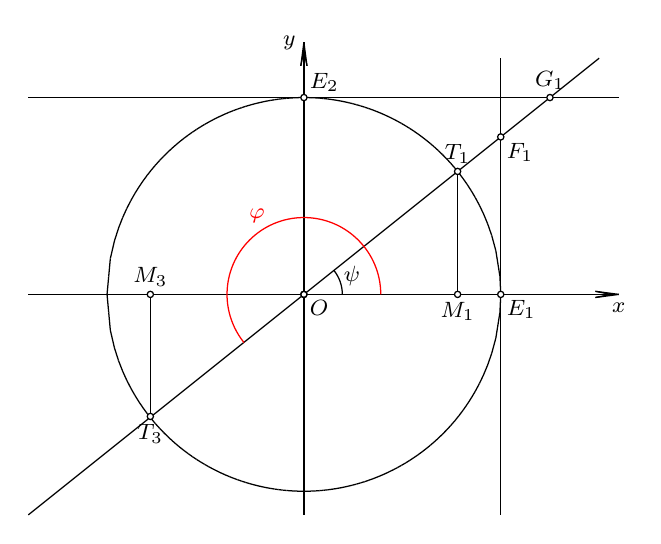
\begin{tikzpicture}
                            % \clip (0,0) rectangle (14.000000,10.000000);
                            {\footnotesize
                            
                            % Drawing 2D Cartesian system
                            \draw [line width=0.016cm] (4.000000,4.000000) circle (0.040000);%
                            % \draw (4.000000,4.000000) node [anchor=north east] { $0$ };%
                            \draw (8.000000,4.000000) node [anchor=north] { $x$ };%
                            \draw (4.000000,7.200000) node [anchor=east] { $y$ };%
                            \draw [line width=0.016cm] (0.500000,4.000000) -- (2.010000,4.000000);%
                            \draw [line width=0.016cm] (2.090000,4.000000) -- (3.960000,4.000000);%
                            \draw [line width=0.016cm] (4.040000,4.000000) -- (5.912172,4.000000);%
                            \draw [line width=0.016cm] (5.992172,4.000000) -- (6.460000,4.000000);%
                            \draw [line width=0.016cm] (6.540000,4.000000) -- (8.000000,4.000000);%
                            \draw [line width=0.016cm] (7.702567,4.039158) -- (8.000000,4.000000);%
                            \draw [line width=0.016cm] (7.702567,4.039158) -- (7.900000,4.000000);%
                            \draw [line width=0.016cm] (7.702567,3.960842) -- (8.000000,4.000000);%
                            \draw [line width=0.016cm] (7.702567,3.960842) -- (7.900000,4.000000);%
                            \draw [line width=0.016cm] (4.000000,1.200000) -- (4.000000,3.960000);%
                            \draw [line width=0.016cm] (4.000000,4.040000) -- (4.000000,6.460000);%
                            \draw [line width=0.016cm] (4.000000,6.540000) -- (4.000000,7.200000);%
                            \draw [line width=0.016cm] (3.960842,6.902567) -- (4.000000,7.200000);%
                            \draw [line width=0.016cm] (3.960842,6.902567) -- (4.000000,7.100000);%
                            \draw [line width=0.016cm] (4.039158,6.902567) -- (4.000000,7.200000);%
                            \draw [line width=0.016cm] (4.039158,6.902567) -- (4.000000,7.100000);%
                            
                            % Drawing 2D ang conic k
                            \draw [line width=0.016cm] (1.500000,4.000000) -- (1.520833,4.227265);%
                            \draw [line width=0.016cm] (1.520833,4.227265) -- (1.541667,4.454530);%
                            \draw [line width=0.016cm] (1.500000,4.000000) -- (1.520833,3.772735);%
                            \draw [line width=0.016cm] (1.520833,3.772735) -- (1.541667,3.545470);%
                            \draw [line width=0.016cm] (1.541667,4.454530) -- (1.593750,4.678204);%
                            \draw [line width=0.016cm] (1.541667,3.545470) -- (1.593750,3.321796);%
                            \draw [line width=0.016cm] (1.593750,4.678204) -- (1.645833,4.841368);%
                            \draw [line width=0.016cm] (1.593750,3.321796) -- (1.645833,3.158632);%
                            \draw [line width=0.016cm] (1.645833,4.841368) -- (1.697917,4.974891);%
                            \draw [line width=0.016cm] (1.645833,3.158632) -- (1.697917,3.025109);%
                            \draw [line width=0.016cm] (1.697917,4.974891) -- (1.750000,5.089725);%
                            \draw [line width=0.016cm] (1.697917,3.025109) -- (1.750000,2.910275);%
                            \draw [line width=0.016cm] (1.750000,5.089725) -- (1.802083,5.191286);%
                            \draw [line width=0.016cm] (1.750000,2.910275) -- (1.802083,2.808714);%
                            \draw [line width=0.016cm] (1.802083,5.191286) -- (1.854167,5.282731);%
                            \draw [line width=0.016cm] (1.802083,2.808714) -- (1.854167,2.717269);%
                            \draw [line width=0.016cm] (1.854167,5.282731) -- (1.906250,5.366093);%
                            \draw [line width=0.016cm] (1.854167,2.717269) -- (1.906250,2.633907);%
                            \draw [line width=0.016cm] (1.906250,5.366093) -- (1.958333,5.442774);%
                            \draw [line width=0.016cm] (1.906250,2.633907) -- (1.958333,2.557226);%
                            \draw [line width=0.016cm] (1.958333,5.442774) -- (2.010417,5.513789);%
                            \draw [line width=0.016cm] (1.958333,2.557226) -- (2.010417,2.486211);%
                            \draw [line width=0.016cm] (2.010417,5.513789) -- (2.062500,5.579903);%
                            \draw [line width=0.016cm] (2.010417,2.486211) -- (2.019015,2.475296);%
                            \draw [line width=0.016cm] (2.062500,5.579903) -- (2.114583,5.641708);%
                            \draw [line width=0.016cm] (2.067579,2.414070) -- (2.114583,2.358292);%
                            \draw [line width=0.016cm] (2.114583,5.641708) -- (2.166667,5.699673);%
                            \draw [line width=0.016cm] (2.114583,2.358292) -- (2.166667,2.300327);%
                            \draw [line width=0.016cm] (2.166667,5.699673) -- (2.218750,5.754180);%
                            \draw [line width=0.016cm] (2.166667,2.300327) -- (2.218750,2.245820);%
                            \draw [line width=0.016cm] (2.218750,5.754180) -- (2.270833,5.805542);%
                            \draw [line width=0.016cm] (2.218750,2.245820) -- (2.270833,2.194458);%
                            \draw [line width=0.016cm] (2.270833,5.805542) -- (2.322917,5.854020);%
                            \draw [line width=0.016cm] (2.270833,2.194458) -- (2.322917,2.145980);%
                            \draw [line width=0.016cm] (2.322917,5.854020) -- (2.375000,5.899836);%
                            \draw [line width=0.016cm] (2.322917,2.145980) -- (2.375000,2.100164);%
                            \draw [line width=0.016cm] (2.375000,5.899836) -- (2.427083,5.943176);%
                            \draw [line width=0.016cm] (2.375000,2.100164) -- (2.427083,2.056824);%
                            \draw [line width=0.016cm] (2.427083,5.943176) -- (2.479167,5.984204);%
                            \draw [line width=0.016cm] (2.427083,2.056824) -- (2.479167,2.015796);%
                            \draw [line width=0.016cm] (2.479167,5.984204) -- (2.531250,6.023060);%
                            \draw [line width=0.016cm] (2.479167,2.015796) -- (2.531250,1.976940);%
                            \draw [line width=0.016cm] (2.531250,6.023060) -- (2.583333,6.059868);%
                            \draw [line width=0.016cm] (2.531250,1.976940) -- (2.583333,1.940132);%
                            \draw [line width=0.016cm] (2.583333,6.059868) -- (2.635417,6.094734);%
                            \draw [line width=0.016cm] (2.583333,1.940132) -- (2.635417,1.905266);%
                            \draw [line width=0.016cm] (2.635417,6.094734) -- (2.687500,6.127756);%
                            \draw [line width=0.016cm] (2.635417,1.905266) -- (2.687500,1.872244);%
                            \draw [line width=0.016cm] (2.687500,6.127756) -- (2.739583,6.159016);%
                            \draw [line width=0.016cm] (2.687500,1.872244) -- (2.739583,1.840984);%
                            \draw [line width=0.016cm] (2.739583,6.159016) -- (2.791667,6.188591);%
                            \draw [line width=0.016cm] (2.739583,1.840984) -- (2.791667,1.811409);%
                            \draw [line width=0.016cm] (2.791667,6.188591) -- (2.843750,6.216548);%
                            \draw [line width=0.016cm] (2.791667,1.811409) -- (2.843750,1.783452);%
                            \draw [line width=0.016cm] (2.843750,6.216548) -- (2.895833,6.242948);%
                            \draw [line width=0.016cm] (2.843750,1.783452) -- (2.895833,1.757052);%
                            \draw [line width=0.016cm] (2.895833,6.242948) -- (2.947917,6.267845);%
                            \draw [line width=0.016cm] (2.895833,1.757052) -- (2.947917,1.732155);%
                            \draw [line width=0.016cm] (2.947917,6.267845) -- (3.000000,6.291288);%
                            \draw [line width=0.016cm] (2.947917,1.732155) -- (3.000000,1.708712);%
                            \draw [line width=0.016cm] (3.000000,6.291288) -- (3.052083,6.313321);%
                            \draw [line width=0.016cm] (3.000000,1.708712) -- (3.052083,1.686679);%
                            \draw [line width=0.016cm] (3.052083,6.313321) -- (3.104167,6.333984);%
                            \draw [line width=0.016cm] (3.052083,1.686679) -- (3.104167,1.666016);%
                            \draw [line width=0.016cm] (3.104167,6.333984) -- (3.156250,6.353314);%
                            \draw [line width=0.016cm] (3.104167,1.666016) -- (3.156250,1.646686);%
                            \draw [line width=0.016cm] (3.156250,6.353314) -- (3.208333,6.371342);%
                            \draw [line width=0.016cm] (3.156250,1.646686) -- (3.208333,1.628658);%
                            \draw [line width=0.016cm] (3.208333,6.371342) -- (3.260417,6.388099);%
                            \draw [line width=0.016cm] (3.208333,1.628658) -- (3.260417,1.611901);%
                            \draw [line width=0.016cm] (3.260417,6.388099) -- (3.312500,6.403611);%
                            \draw [line width=0.016cm] (3.260417,1.611901) -- (3.312500,1.596389);%
                            \draw [line width=0.016cm] (3.312500,6.403611) -- (3.364583,6.417901);%
                            \draw [line width=0.016cm] (3.312500,1.596389) -- (3.364583,1.582099);%
                            \draw [line width=0.016cm] (3.364583,6.417901) -- (3.416667,6.430992);%
                            \draw [line width=0.016cm] (3.364583,1.582099) -- (3.416667,1.569008);%
                            \draw [line width=0.016cm] (3.416667,6.430992) -- (3.468750,6.442903);%
                            \draw [line width=0.016cm] (3.416667,1.569008) -- (3.468750,1.557097);%
                            \draw [line width=0.016cm] (3.468750,6.442903) -- (3.520833,6.453650);%
                            \draw [line width=0.016cm] (3.468750,1.557097) -- (3.520833,1.546350);%
                            \draw [line width=0.016cm] (3.520833,6.453650) -- (3.572917,6.463250);%
                            \draw [line width=0.016cm] (3.520833,1.546350) -- (3.572917,1.536750);%
                            \draw [line width=0.016cm] (3.572917,6.463250) -- (3.625000,6.471715);%
                            \draw [line width=0.016cm] (3.572917,1.536750) -- (3.625000,1.528285);%
                            \draw [line width=0.016cm] (3.625000,6.471715) -- (3.677083,6.479057);%
                            \draw [line width=0.016cm] (3.625000,1.528285) -- (3.677083,1.520943);%
                            \draw [line width=0.016cm] (3.677083,6.479057) -- (3.729167,6.485287);%
                            \draw [line width=0.016cm] (3.677083,1.520943) -- (3.729167,1.514713);%
                            \draw [line width=0.016cm] (3.729167,6.485287) -- (3.781250,6.490411);%
                            \draw [line width=0.016cm] (3.729167,1.514713) -- (3.781250,1.509589);%
                            \draw [line width=0.016cm] (3.781250,6.490411) -- (3.833333,6.494438);%
                            \draw [line width=0.016cm] (3.781250,1.509589) -- (3.833333,1.505562);%
                            \draw [line width=0.016cm] (3.833333,6.494438) -- (3.885417,6.497373);%
                            \draw [line width=0.016cm] (3.833333,1.505562) -- (3.885417,1.502627);%
                            \draw [line width=0.016cm] (3.885417,6.497373) -- (3.937500,6.499219);%
                            \draw [line width=0.016cm] (3.885417,1.502627) -- (3.937500,1.500781);%
                            \draw [line width=0.016cm] (3.937500,6.499219) -- (3.960003,6.499547);%
                            \draw [line width=0.016cm] (3.937500,1.500781) -- (3.989583,1.500022);%
                            \draw [line width=0.016cm] (4.039999,6.499663) -- (4.041667,6.499653);%
                            \draw [line width=0.016cm] (3.989583,1.500022) -- (4.041667,1.500347);%
                            \draw [line width=0.016cm] (4.041667,6.499653) -- (4.093750,6.498242);%
                            \draw [line width=0.016cm] (4.041667,1.500347) -- (4.093750,1.501758);%
                            \draw [line width=0.016cm] (4.093750,6.498242) -- (4.145833,6.495743);%
                            \draw [line width=0.016cm] (4.093750,1.501758) -- (4.145833,1.504257);%
                            \draw [line width=0.016cm] (4.145833,6.495743) -- (4.197917,6.492153);%
                            \draw [line width=0.016cm] (4.145833,1.504257) -- (4.197917,1.507847);%
                            \draw [line width=0.016cm] (4.197917,6.492153) -- (4.250000,6.487469);%
                            \draw [line width=0.016cm] (4.197917,1.507847) -- (4.250000,1.512531);%
                            \draw [line width=0.016cm] (4.250000,6.487469) -- (4.302083,6.481682);%
                            \draw [line width=0.016cm] (4.250000,1.512531) -- (4.302083,1.518318);%
                            \draw [line width=0.016cm] (4.302083,6.481682) -- (4.354167,6.474786);%
                            \draw [line width=0.016cm] (4.302083,1.518318) -- (4.354167,1.525214);%
                            \draw [line width=0.016cm] (4.354167,6.474786) -- (4.406250,6.466771);%
                            \draw [line width=0.016cm] (4.354167,1.525214) -- (4.406250,1.533229);%
                            \draw [line width=0.016cm] (4.406250,6.466771) -- (4.458333,6.457627);%
                            \draw [line width=0.016cm] (4.406250,1.533229) -- (4.458333,1.542373);%
                            \draw [line width=0.016cm] (4.458333,6.457627) -- (4.510417,6.447340);%
                            \draw [line width=0.016cm] (4.458333,1.542373) -- (4.510417,1.552660);%
                            \draw [line width=0.016cm] (4.510417,6.447340) -- (4.562500,6.435897);%
                            \draw [line width=0.016cm] (4.510417,1.552660) -- (4.562500,1.564103);%
                            \draw [line width=0.016cm] (4.562500,6.435897) -- (4.614583,6.423280);%
                            \draw [line width=0.016cm] (4.562500,1.564103) -- (4.614583,1.576720);%
                            \draw [line width=0.016cm] (4.614583,6.423280) -- (4.666667,6.409472);%
                            \draw [line width=0.016cm] (4.614583,1.576720) -- (4.666667,1.590528);%
                            \draw [line width=0.016cm] (4.666667,6.409472) -- (4.718750,6.394452);%
                            \draw [line width=0.016cm] (4.666667,1.590528) -- (4.718750,1.605548);%
                            \draw [line width=0.016cm] (4.718750,6.394452) -- (4.770833,6.378196);%
                            \draw [line width=0.016cm] (4.718750,1.605548) -- (4.770833,1.621804);%
                            \draw [line width=0.016cm] (4.770833,6.378196) -- (4.822917,6.360680);%
                            \draw [line width=0.016cm] (4.770833,1.621804) -- (4.822917,1.639320);%
                            \draw [line width=0.016cm] (4.822917,6.360680) -- (4.875000,6.341874);%
                            \draw [line width=0.016cm] (4.822917,1.639320) -- (4.875000,1.658126);%
                            \draw [line width=0.016cm] (4.875000,6.341874) -- (4.927083,6.321749);%
                            \draw [line width=0.016cm] (4.875000,1.658126) -- (4.927083,1.678251);%
                            \draw [line width=0.016cm] (4.927083,6.321749) -- (4.979167,6.300268);%
                            \draw [line width=0.016cm] (4.927083,1.678251) -- (4.979167,1.699732);%
                            \draw [line width=0.016cm] (4.979167,6.300268) -- (5.031250,6.277394);%
                            \draw [line width=0.016cm] (4.979167,1.699732) -- (5.031250,1.722606);%
                            \draw [line width=0.016cm] (5.031250,6.277394) -- (5.083333,6.253084);%
                            \draw [line width=0.016cm] (5.031250,1.722606) -- (5.083333,1.746916);%
                            \draw [line width=0.016cm] (5.083333,6.253084) -- (5.135417,6.227292);%
                            \draw [line width=0.016cm] (5.083333,1.746916) -- (5.135417,1.772708);%
                            \draw [line width=0.016cm] (5.135417,6.227292) -- (5.187500,6.199964);%
                            \draw [line width=0.016cm] (5.135417,1.772708) -- (5.187500,1.800036);%
                            \draw [line width=0.016cm] (5.187500,6.199964) -- (5.239583,6.171044);%
                            \draw [line width=0.016cm] (5.187500,1.800036) -- (5.239583,1.828956);%
                            \draw [line width=0.016cm] (5.239583,6.171044) -- (5.291667,6.140467);%
                            \draw [line width=0.016cm] (5.239583,1.828956) -- (5.291667,1.859533);%
                            \draw [line width=0.016cm] (5.291667,6.140467) -- (5.343750,6.108159);%
                            \draw [line width=0.016cm] (5.291667,1.859533) -- (5.343750,1.891841);%
                            \draw [line width=0.016cm] (5.343750,6.108159) -- (5.395833,6.074042);%
                            \draw [line width=0.016cm] (5.343750,1.891841) -- (5.395833,1.925958);%
                            \draw [line width=0.016cm] (5.395833,6.074042) -- (5.447917,6.038023);%
                            \draw [line width=0.016cm] (5.395833,1.925958) -- (5.447917,1.961977);%
                            \draw [line width=0.016cm] (5.447917,6.038023) -- (5.500000,6.000000);%
                            \draw [line width=0.016cm] (5.447917,1.961977) -- (5.500000,2.000000);%
                            \draw [line width=0.016cm] (5.500000,6.000000) -- (5.552083,5.959856);%
                            \draw [line width=0.016cm] (5.500000,2.000000) -- (5.552083,2.040144);%
                            \draw [line width=0.016cm] (5.552083,5.959856) -- (5.604167,5.917459);%
                            \draw [line width=0.016cm] (5.552083,2.040144) -- (5.604167,2.082541);%
                            \draw [line width=0.016cm] (5.604167,5.917459) -- (5.656250,5.872655);%
                            \draw [line width=0.016cm] (5.604167,2.082541) -- (5.656250,2.127345);%
                            \draw [line width=0.016cm] (5.656250,5.872655) -- (5.708333,5.825266);%
                            \draw [line width=0.016cm] (5.656250,2.127345) -- (5.708333,2.174734);%
                            \draw [line width=0.016cm] (5.708333,5.825266) -- (5.760417,5.775087);%
                            \draw [line width=0.016cm] (5.708333,2.174734) -- (5.760417,2.224913);%
                            \draw [line width=0.016cm] (5.760417,5.775087) -- (5.812500,5.721872);%
                            \draw [line width=0.016cm] (5.760417,2.224913) -- (5.812500,2.278128);%
                            \draw [line width=0.016cm] (5.812500,5.721872) -- (5.864583,5.665331);%
                            \draw [line width=0.016cm] (5.812500,2.278128) -- (5.864583,2.334669);%
                            \draw [line width=0.016cm] (5.864583,5.665331) -- (5.916667,5.605113);%
                            \draw [line width=0.016cm] (5.864583,2.334669) -- (5.916667,2.394887);%
                            \draw [line width=0.016cm] (5.916667,5.605113) -- (5.926769,5.592636);%
                            \draw [line width=0.016cm] (5.916667,2.394887) -- (5.968750,2.459213);%
                            \draw [line width=0.016cm] (5.976756,5.530184) -- (6.020833,5.471813);%
                            \draw [line width=0.016cm] (5.968750,2.459213) -- (6.020833,2.528187);%
                            \draw [line width=0.016cm] (6.020833,5.471813) -- (6.072917,5.397504);%
                            \draw [line width=0.016cm] (6.020833,2.528187) -- (6.072917,2.602496);%
                            \draw [line width=0.016cm] (6.072917,5.397504) -- (6.125000,5.316957);%
                            \draw [line width=0.016cm] (6.072917,2.602496) -- (6.125000,2.683043);%
                            \draw [line width=0.016cm] (6.125000,5.316957) -- (6.177083,5.228946);%
                            \draw [line width=0.016cm] (6.125000,2.683043) -- (6.177083,2.771054);%
                            \draw [line width=0.016cm] (6.177083,5.228946) -- (6.229167,5.131731);%
                            \draw [line width=0.016cm] (6.177083,2.771054) -- (6.229167,2.868269);%
                            \draw [line width=0.016cm] (6.229167,5.131731) -- (6.281250,5.022692);%
                            \draw [line width=0.016cm] (6.229167,2.868269) -- (6.281250,2.977308);%
                            \draw [line width=0.016cm] (6.281250,5.022692) -- (6.333333,4.897527);%
                            \draw [line width=0.016cm] (6.281250,2.977308) -- (6.333333,3.102473);%
                            \draw [line width=0.016cm] (6.333333,4.897527) -- (6.385417,4.748189);%
                            \draw [line width=0.016cm] (6.333333,3.102473) -- (6.385417,3.251811);%
                            \draw [line width=0.016cm] (6.385417,4.748189) -- (6.437500,4.555512);%
                            \draw [line width=0.016cm] (6.385417,3.251811) -- (6.437500,3.444488);%
                            \draw [line width=0.016cm] (6.437500,4.555512) -- (6.489583,4.227980);%
                            \draw [line width=0.016cm] (6.437500,3.444488) -- (6.489583,3.772020);%
                            \draw [line width=0.016cm] (6.498174,4.039958) -- (6.494792,4.113990);%
                            \draw [line width=0.016cm] (6.494792,4.113990) -- (6.489583,4.227980);%
                            \draw [line width=0.016cm] (6.498174,3.960042) -- (6.494792,3.886010);%
                            \draw [line width=0.016cm] (6.494792,3.886010) -- (6.489583,3.772020);%
                            
                            % Drawing line l
                            \draw [line width=0.016cm] (0.500000,1.200000) -- (2.024244,2.419395);%
                            \draw [line width=0.016cm] (2.085512,2.468409) -- (3.968765,3.975012);%
                            \draw [line width=0.016cm] (4.031235,4.024988) -- (5.920937,5.536750);%
                            \draw [line width=0.016cm] (5.983407,5.586725) -- (6.468765,5.975012);%
                            \draw [line width=0.016cm] (6.531235,6.024988) -- (7.093765,6.475012);%
                            \draw [line width=0.016cm] (7.156235,6.524988) -- (7.750000,7.000000);%
                            
                            % Marking point \psi
                            \draw (4.400000,4.000000) node [anchor=south west] { $\psi$ };%
                            
                            % Marking point O by circle
                            \draw [line width=0.016cm] (4.000000,4.000000) circle (0.040000);%
                            \draw (3.970000,4.030000) node [anchor=north west] { $O$ };%
                            
                            % Marking point M_1 by circle
                            \draw [line width=0.016cm] (5.952172,4.000000) circle (0.040000);%
                            \draw (5.952172,4.000000) node [anchor=north] { $M_1$ };%
                            
                            % Marking point M_3 by circle
                            \draw [line width=0.016cm] (2.050000,4.000000) circle (0.040000);%
                            \draw (2.050000,4.000000) node [anchor=south] { $M_3$ };%
                            
                            % Marking point T_1 by circle
                            \draw [line width=0.016cm] (5.952172,5.561738) circle (0.040000);%
                            \draw (5.952172,5.561738) node [anchor=south] { $T_1$ };%
                            
                            % Marking point T_3 by circle
                            \draw [line width=0.016cm] (2.050000,2.450000) circle (0.040000);%
                            \draw (2.050000,2.450000) node [anchor=north] { $T_3$ };%
                            
                            % Marking point E_1 by circle
                            \draw [line width=0.016cm] (6.500000,4.000000) circle (0.040000);%
                            \draw (6.470000,4.030000) node [anchor=north west] { $E_1$ };%
                            
                            % Marking point E_2 by circle
                            \draw [line width=0.016cm] (4.000000,6.500000) circle (0.040000);%
                            \draw (3.970000,6.470000) node [anchor=south west] { $E_2$ };%
                            
                            % Drawing line y
                            \draw [line width=0.016cm] (0.500000,6.500000) -- (3.960000,6.500000);%
                            \draw [line width=0.016cm] (4.040000,6.500000) -- (7.085000,6.500000);%
                            \draw [line width=0.016cm] (7.165000,6.500000) -- (8.000000,6.500000);%
                            
                            % Marking point G_1 by circle
                            \draw [line width=0.016cm] (7.125000,6.500000) circle (0.040000);%
                            \draw (7.125000,6.500000) node [anchor=south] { $G_1$ };%
                            
                            % Marking point F_1 by circle
                            \draw [line width=0.016cm] (6.500000,6.000000) circle (0.040000);%
                            \draw (6.470000,6.030000) node [anchor=north west] { $F_1$ };%
                            
                            % Drawing line z
                            \draw [line width=0.016cm] (6.500000,1.200000) -- (6.500000,3.960000);%
                            \draw [line width=0.016cm] (6.500000,4.040000) -- (6.500000,5.960000);%
                            \draw [line width=0.016cm] (6.500000,6.040000) -- (6.500000,7.000000);%
                            
                            % Drawing segment T_3 M_3
                            \draw [line width=0.016cm] (2.050000,2.490000) -- (2.050000,3.960000);%
                            
                            % Drawing segment T_1 M_1
                            \draw [line width=0.016cm] (5.952172,5.521738) -- (5.952172,4.040000);%
                            
                            % Drawing arc O J 38.66
                            \draw [line width=0.016cm] (4.488043,4.000000) arc (360:360:0.488043 and 0.488043) --(4.488043,4.000000) arc (0:38:0.488043 and 0.488043) -- (4.381098,4.304878);%
                            
                            % Changing color 255 0 0
                            \definecolor{r255g0b0}{rgb}{1.000000,0.000000,0.000000}%
                            \color{r255g0b0}% 
                            
                            % Drawing arc O I 218.84
                            \draw [line width=0.016cm] (4.976086,4.000000) arc (360:360:0.976086 and 0.976086) --(4.976086,4.000000) arc (0:218:0.976086 and 0.976086) -- (3.239726,3.387850);%
                            
                            % Marking point \varphi
                            \draw (3.200000,4.800000) node [anchor=south west] { $\varphi$ };%
                            \color{black}
                            }
                        \end{tikzpicture}                          
                    \end{figure}

                   \column{0.43\textwidth}     
                        \begin{alertblock}{}
                            Sinusa in kosinusa kotov, ki se razlikujeta za $\pi$, sta nasprotno enaka. 
                            $$ \sin\left(\pi+\psi\right) = -\sin\psi $$
                            $$ \cos\left(\pi+\psi\right) = -\cos\psi $$
                            
                        \end{alertblock}

                        \begin{alertblock}{}
                            Tangensa in kotangensa kotov, ki se razlikujeta za $\pi$, sta enaka.
                            $$ \tan\left(\pi+\psi\right) = \tan\psi $$
                            $$ \cot\left(\pi+\psi\right) = \cot\psi $$        
                        \end{alertblock}      
        
        \end{columns}


        \end{frame}

        \begin{frame}
            \large\textbf{Kot med $\frac{3\pi}{2}$ in $2\pi$}
            ~\\
            \normalsize

            \begin{columns}

                \column{0.55\textwidth}
                    \begin{figure}
                        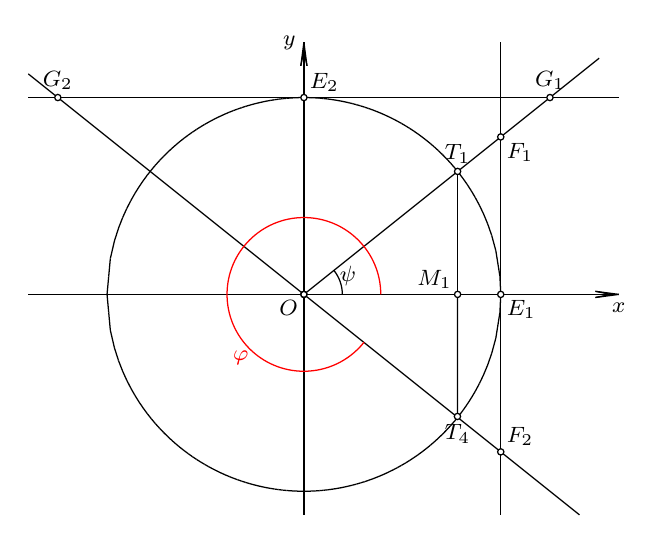
\begin{tikzpicture}
                            % \clip (0,0) rectangle (14.000000,10.000000);
                            {\footnotesize
                            
                            % Drawing 2D Cartesian system
                            \draw [line width=0.016cm] (4.000000,4.000000) circle (0.040000);%
                            % \draw (4.000000,4.000000) node [anchor=north east] { $0$ };%
                            \draw (8.000000,4.000000) node [anchor=north] { $x$ };%
                            \draw (4.000000,7.200000) node [anchor=east] { $y$ };%
                            \draw [line width=0.016cm] (0.500000,4.000000) -- (3.960000,4.000000);%
                            \draw [line width=0.016cm] (4.040000,4.000000) -- (5.912172,4.000000);%
                            \draw [line width=0.016cm] (5.992172,4.000000) -- (6.460000,4.000000);%
                            \draw [line width=0.016cm] (6.540000,4.000000) -- (8.000000,4.000000);%
                            \draw [line width=0.016cm] (7.702567,4.039158) -- (8.000000,4.000000);%
                            \draw [line width=0.016cm] (7.702567,4.039158) -- (7.900000,4.000000);%
                            \draw [line width=0.016cm] (7.702567,3.960842) -- (8.000000,4.000000);%
                            \draw [line width=0.016cm] (7.702567,3.960842) -- (7.900000,4.000000);%
                            \draw [line width=0.016cm] (4.000000,1.200000) -- (4.000000,3.960000);%
                            \draw [line width=0.016cm] (4.000000,4.040000) -- (4.000000,6.460000);%
                            \draw [line width=0.016cm] (4.000000,6.540000) -- (4.000000,7.200000);%
                            \draw [line width=0.016cm] (3.960842,6.902567) -- (4.000000,7.200000);%
                            \draw [line width=0.016cm] (3.960842,6.902567) -- (4.000000,7.100000);%
                            \draw [line width=0.016cm] (4.039158,6.902567) -- (4.000000,7.200000);%
                            \draw [line width=0.016cm] (4.039158,6.902567) -- (4.000000,7.100000);%
                            
                            % Drawing 2D ang conic k
                            \draw [line width=0.016cm] (1.500000,4.000000) -- (1.520833,4.227265);%
                            \draw [line width=0.016cm] (1.520833,4.227265) -- (1.541667,4.454530);%
                            \draw [line width=0.016cm] (1.500000,4.000000) -- (1.520833,3.772735);%
                            \draw [line width=0.016cm] (1.520833,3.772735) -- (1.541667,3.545470);%
                            \draw [line width=0.016cm] (1.541667,4.454530) -- (1.593750,4.678204);%
                            \draw [line width=0.016cm] (1.541667,3.545470) -- (1.593750,3.321796);%
                            \draw [line width=0.016cm] (1.593750,4.678204) -- (1.645833,4.841368);%
                            \draw [line width=0.016cm] (1.593750,3.321796) -- (1.645833,3.158632);%
                            \draw [line width=0.016cm] (1.645833,4.841368) -- (1.697917,4.974891);%
                            \draw [line width=0.016cm] (1.645833,3.158632) -- (1.697917,3.025109);%
                            \draw [line width=0.016cm] (1.697917,4.974891) -- (1.750000,5.089725);%
                            \draw [line width=0.016cm] (1.697917,3.025109) -- (1.750000,2.910275);%
                            \draw [line width=0.016cm] (1.750000,5.089725) -- (1.802083,5.191286);%
                            \draw [line width=0.016cm] (1.750000,2.910275) -- (1.802083,2.808714);%
                            \draw [line width=0.016cm] (1.802083,5.191286) -- (1.854167,5.282731);%
                            \draw [line width=0.016cm] (1.802083,2.808714) -- (1.854167,2.717269);%
                            \draw [line width=0.016cm] (1.854167,5.282731) -- (1.906250,5.366093);%
                            \draw [line width=0.016cm] (1.854167,2.717269) -- (1.906250,2.633907);%
                            \draw [line width=0.016cm] (1.906250,5.366093) -- (1.958333,5.442774);%
                            \draw [line width=0.016cm] (1.906250,2.633907) -- (1.958333,2.557226);%
                            \draw [line width=0.016cm] (1.958333,5.442774) -- (2.010417,5.513789);%
                            \draw [line width=0.016cm] (1.958333,2.557226) -- (2.010417,2.486211);%
                            \draw [line width=0.016cm] (2.010417,5.513789) -- (2.062500,5.579903);%
                            \draw [line width=0.016cm] (2.010417,2.486211) -- (2.062500,2.420097);%
                            \draw [line width=0.016cm] (2.062500,5.579903) -- (2.114583,5.641708);%
                            \draw [line width=0.016cm] (2.062500,2.420097) -- (2.114583,2.358292);%
                            \draw [line width=0.016cm] (2.114583,5.641708) -- (2.166667,5.699673);%
                            \draw [line width=0.016cm] (2.114583,2.358292) -- (2.166667,2.300327);%
                            \draw [line width=0.016cm] (2.166667,5.699673) -- (2.218750,5.754180);%
                            \draw [line width=0.016cm] (2.166667,2.300327) -- (2.218750,2.245820);%
                            \draw [line width=0.016cm] (2.218750,5.754180) -- (2.270833,5.805542);%
                            \draw [line width=0.016cm] (2.218750,2.245820) -- (2.270833,2.194458);%
                            \draw [line width=0.016cm] (2.270833,5.805542) -- (2.322917,5.854020);%
                            \draw [line width=0.016cm] (2.270833,2.194458) -- (2.322917,2.145980);%
                            \draw [line width=0.016cm] (2.322917,5.854020) -- (2.375000,5.899836);%
                            \draw [line width=0.016cm] (2.322917,2.145980) -- (2.375000,2.100164);%
                            \draw [line width=0.016cm] (2.375000,5.899836) -- (2.427083,5.943176);%
                            \draw [line width=0.016cm] (2.375000,2.100164) -- (2.427083,2.056824);%
                            \draw [line width=0.016cm] (2.427083,5.943176) -- (2.479167,5.984204);%
                            \draw [line width=0.016cm] (2.427083,2.056824) -- (2.479167,2.015796);%
                            \draw [line width=0.016cm] (2.479167,5.984204) -- (2.531250,6.023060);%
                            \draw [line width=0.016cm] (2.479167,2.015796) -- (2.531250,1.976940);%
                            \draw [line width=0.016cm] (2.531250,6.023060) -- (2.583333,6.059868);%
                            \draw [line width=0.016cm] (2.531250,1.976940) -- (2.583333,1.940132);%
                            \draw [line width=0.016cm] (2.583333,6.059868) -- (2.635417,6.094734);%
                            \draw [line width=0.016cm] (2.583333,1.940132) -- (2.635417,1.905266);%
                            \draw [line width=0.016cm] (2.635417,6.094734) -- (2.687500,6.127756);%
                            \draw [line width=0.016cm] (2.635417,1.905266) -- (2.687500,1.872244);%
                            \draw [line width=0.016cm] (2.687500,6.127756) -- (2.739583,6.159016);%
                            \draw [line width=0.016cm] (2.687500,1.872244) -- (2.739583,1.840984);%
                            \draw [line width=0.016cm] (2.739583,6.159016) -- (2.791667,6.188591);%
                            \draw [line width=0.016cm] (2.739583,1.840984) -- (2.791667,1.811409);%
                            \draw [line width=0.016cm] (2.791667,6.188591) -- (2.843750,6.216548);%
                            \draw [line width=0.016cm] (2.791667,1.811409) -- (2.843750,1.783452);%
                            \draw [line width=0.016cm] (2.843750,6.216548) -- (2.895833,6.242948);%
                            \draw [line width=0.016cm] (2.843750,1.783452) -- (2.895833,1.757052);%
                            \draw [line width=0.016cm] (2.895833,6.242948) -- (2.947917,6.267845);%
                            \draw [line width=0.016cm] (2.895833,1.757052) -- (2.947917,1.732155);%
                            \draw [line width=0.016cm] (2.947917,6.267845) -- (3.000000,6.291288);%
                            \draw [line width=0.016cm] (2.947917,1.732155) -- (3.000000,1.708712);%
                            \draw [line width=0.016cm] (3.000000,6.291288) -- (3.052083,6.313321);%
                            \draw [line width=0.016cm] (3.000000,1.708712) -- (3.052083,1.686679);%
                            \draw [line width=0.016cm] (3.052083,6.313321) -- (3.104167,6.333984);%
                            \draw [line width=0.016cm] (3.052083,1.686679) -- (3.104167,1.666016);%
                            \draw [line width=0.016cm] (3.104167,6.333984) -- (3.156250,6.353314);%
                            \draw [line width=0.016cm] (3.104167,1.666016) -- (3.156250,1.646686);%
                            \draw [line width=0.016cm] (3.156250,6.353314) -- (3.208333,6.371342);%
                            \draw [line width=0.016cm] (3.156250,1.646686) -- (3.208333,1.628658);%
                            \draw [line width=0.016cm] (3.208333,6.371342) -- (3.260417,6.388099);%
                            \draw [line width=0.016cm] (3.208333,1.628658) -- (3.260417,1.611901);%
                            \draw [line width=0.016cm] (3.260417,6.388099) -- (3.312500,6.403611);%
                            \draw [line width=0.016cm] (3.260417,1.611901) -- (3.312500,1.596389);%
                            \draw [line width=0.016cm] (3.312500,6.403611) -- (3.364583,6.417901);%
                            \draw [line width=0.016cm] (3.312500,1.596389) -- (3.364583,1.582099);%
                            \draw [line width=0.016cm] (3.364583,6.417901) -- (3.416667,6.430992);%
                            \draw [line width=0.016cm] (3.364583,1.582099) -- (3.416667,1.569008);%
                            \draw [line width=0.016cm] (3.416667,6.430992) -- (3.468750,6.442903);%
                            \draw [line width=0.016cm] (3.416667,1.569008) -- (3.468750,1.557097);%
                            \draw [line width=0.016cm] (3.468750,6.442903) -- (3.520833,6.453650);%
                            \draw [line width=0.016cm] (3.468750,1.557097) -- (3.520833,1.546350);%
                            \draw [line width=0.016cm] (3.520833,6.453650) -- (3.572917,6.463250);%
                            \draw [line width=0.016cm] (3.520833,1.546350) -- (3.572917,1.536750);%
                            \draw [line width=0.016cm] (3.572917,6.463250) -- (3.625000,6.471715);%
                            \draw [line width=0.016cm] (3.572917,1.536750) -- (3.625000,1.528285);%
                            \draw [line width=0.016cm] (3.625000,6.471715) -- (3.677083,6.479057);%
                            \draw [line width=0.016cm] (3.625000,1.528285) -- (3.677083,1.520943);%
                            \draw [line width=0.016cm] (3.677083,6.479057) -- (3.729167,6.485287);%
                            \draw [line width=0.016cm] (3.677083,1.520943) -- (3.729167,1.514713);%
                            \draw [line width=0.016cm] (3.729167,6.485287) -- (3.781250,6.490411);%
                            \draw [line width=0.016cm] (3.729167,1.514713) -- (3.781250,1.509589);%
                            \draw [line width=0.016cm] (3.781250,6.490411) -- (3.833333,6.494438);%
                            \draw [line width=0.016cm] (3.781250,1.509589) -- (3.833333,1.505562);%
                            \draw [line width=0.016cm] (3.833333,6.494438) -- (3.885417,6.497373);%
                            \draw [line width=0.016cm] (3.833333,1.505562) -- (3.885417,1.502627);%
                            \draw [line width=0.016cm] (3.885417,6.497373) -- (3.937500,6.499219);%
                            \draw [line width=0.016cm] (3.885417,1.502627) -- (3.937500,1.500781);%
                            \draw [line width=0.016cm] (3.937500,6.499219) -- (3.960003,6.499547);%
                            \draw [line width=0.016cm] (3.937500,1.500781) -- (3.989583,1.500022);%
                            \draw [line width=0.016cm] (4.039999,6.499663) -- (4.041667,6.499653);%
                            \draw [line width=0.016cm] (3.989583,1.500022) -- (4.041667,1.500347);%
                            \draw [line width=0.016cm] (4.041667,6.499653) -- (4.093750,6.498242);%
                            \draw [line width=0.016cm] (4.041667,1.500347) -- (4.093750,1.501758);%
                            \draw [line width=0.016cm] (4.093750,6.498242) -- (4.145833,6.495743);%
                            \draw [line width=0.016cm] (4.093750,1.501758) -- (4.145833,1.504257);%
                            \draw [line width=0.016cm] (4.145833,6.495743) -- (4.197917,6.492153);%
                            \draw [line width=0.016cm] (4.145833,1.504257) -- (4.197917,1.507847);%
                            \draw [line width=0.016cm] (4.197917,6.492153) -- (4.250000,6.487469);%
                            \draw [line width=0.016cm] (4.197917,1.507847) -- (4.250000,1.512531);%
                            \draw [line width=0.016cm] (4.250000,6.487469) -- (4.302083,6.481682);%
                            \draw [line width=0.016cm] (4.250000,1.512531) -- (4.302083,1.518318);%
                            \draw [line width=0.016cm] (4.302083,6.481682) -- (4.354167,6.474786);%
                            \draw [line width=0.016cm] (4.302083,1.518318) -- (4.354167,1.525214);%
                            \draw [line width=0.016cm] (4.354167,6.474786) -- (4.406250,6.466771);%
                            \draw [line width=0.016cm] (4.354167,1.525214) -- (4.406250,1.533229);%
                            \draw [line width=0.016cm] (4.406250,6.466771) -- (4.458333,6.457627);%
                            \draw [line width=0.016cm] (4.406250,1.533229) -- (4.458333,1.542373);%
                            \draw [line width=0.016cm] (4.458333,6.457627) -- (4.510417,6.447340);%
                            \draw [line width=0.016cm] (4.458333,1.542373) -- (4.510417,1.552660);%
                            \draw [line width=0.016cm] (4.510417,6.447340) -- (4.562500,6.435897);%
                            \draw [line width=0.016cm] (4.510417,1.552660) -- (4.562500,1.564103);%
                            \draw [line width=0.016cm] (4.562500,6.435897) -- (4.614583,6.423280);%
                            \draw [line width=0.016cm] (4.562500,1.564103) -- (4.614583,1.576720);%
                            \draw [line width=0.016cm] (4.614583,6.423280) -- (4.666667,6.409472);%
                            \draw [line width=0.016cm] (4.614583,1.576720) -- (4.666667,1.590528);%
                            \draw [line width=0.016cm] (4.666667,6.409472) -- (4.718750,6.394452);%
                            \draw [line width=0.016cm] (4.666667,1.590528) -- (4.718750,1.605548);%
                            \draw [line width=0.016cm] (4.718750,6.394452) -- (4.770833,6.378196);%
                            \draw [line width=0.016cm] (4.718750,1.605548) -- (4.770833,1.621804);%
                            \draw [line width=0.016cm] (4.770833,6.378196) -- (4.822917,6.360680);%
                            \draw [line width=0.016cm] (4.770833,1.621804) -- (4.822917,1.639320);%
                            \draw [line width=0.016cm] (4.822917,6.360680) -- (4.875000,6.341874);%
                            \draw [line width=0.016cm] (4.822917,1.639320) -- (4.875000,1.658126);%
                            \draw [line width=0.016cm] (4.875000,6.341874) -- (4.927083,6.321749);%
                            \draw [line width=0.016cm] (4.875000,1.658126) -- (4.927083,1.678251);%
                            \draw [line width=0.016cm] (4.927083,6.321749) -- (4.979167,6.300268);%
                            \draw [line width=0.016cm] (4.927083,1.678251) -- (4.979167,1.699732);%
                            \draw [line width=0.016cm] (4.979167,6.300268) -- (5.031250,6.277394);%
                            \draw [line width=0.016cm] (4.979167,1.699732) -- (5.031250,1.722606);%
                            \draw [line width=0.016cm] (5.031250,6.277394) -- (5.083333,6.253084);%
                            \draw [line width=0.016cm] (5.031250,1.722606) -- (5.083333,1.746916);%
                            \draw [line width=0.016cm] (5.083333,6.253084) -- (5.135417,6.227292);%
                            \draw [line width=0.016cm] (5.083333,1.746916) -- (5.135417,1.772708);%
                            \draw [line width=0.016cm] (5.135417,6.227292) -- (5.187500,6.199964);%
                            \draw [line width=0.016cm] (5.135417,1.772708) -- (5.187500,1.800036);%
                            \draw [line width=0.016cm] (5.187500,6.199964) -- (5.239583,6.171044);%
                            \draw [line width=0.016cm] (5.187500,1.800036) -- (5.239583,1.828956);%
                            \draw [line width=0.016cm] (5.239583,6.171044) -- (5.291667,6.140467);%
                            \draw [line width=0.016cm] (5.239583,1.828956) -- (5.291667,1.859533);%
                            \draw [line width=0.016cm] (5.291667,6.140467) -- (5.343750,6.108159);%
                            \draw [line width=0.016cm] (5.291667,1.859533) -- (5.343750,1.891841);%
                            \draw [line width=0.016cm] (5.343750,6.108159) -- (5.395833,6.074042);%
                            \draw [line width=0.016cm] (5.343750,1.891841) -- (5.395833,1.925958);%
                            \draw [line width=0.016cm] (5.395833,6.074042) -- (5.447917,6.038023);%
                            \draw [line width=0.016cm] (5.395833,1.925958) -- (5.447917,1.961977);%
                            \draw [line width=0.016cm] (5.447917,6.038023) -- (5.500000,6.000000);%
                            \draw [line width=0.016cm] (5.447917,1.961977) -- (5.500000,2.000000);%
                            \draw [line width=0.016cm] (5.500000,6.000000) -- (5.552083,5.959856);%
                            \draw [line width=0.016cm] (5.500000,2.000000) -- (5.552083,2.040144);%
                            \draw [line width=0.016cm] (5.552083,5.959856) -- (5.604167,5.917459);%
                            \draw [line width=0.016cm] (5.552083,2.040144) -- (5.604167,2.082541);%
                            \draw [line width=0.016cm] (5.604167,5.917459) -- (5.656250,5.872655);%
                            \draw [line width=0.016cm] (5.604167,2.082541) -- (5.656250,2.127345);%
                            \draw [line width=0.016cm] (5.656250,5.872655) -- (5.708333,5.825266);%
                            \draw [line width=0.016cm] (5.656250,2.127345) -- (5.708333,2.174734);%
                            \draw [line width=0.016cm] (5.708333,5.825266) -- (5.760417,5.775087);%
                            \draw [line width=0.016cm] (5.708333,2.174734) -- (5.760417,2.224913);%
                            \draw [line width=0.016cm] (5.760417,5.775087) -- (5.812500,5.721872);%
                            \draw [line width=0.016cm] (5.760417,2.224913) -- (5.812500,2.278128);%
                            \draw [line width=0.016cm] (5.812500,5.721872) -- (5.864583,5.665331);%
                            \draw [line width=0.016cm] (5.812500,2.278128) -- (5.864583,2.334669);%
                            \draw [line width=0.016cm] (5.864583,5.665331) -- (5.916667,5.605113);%
                            \draw [line width=0.016cm] (5.864583,2.334669) -- (5.916667,2.394887);%
                            \draw [line width=0.016cm] (5.916667,5.605113) -- (5.926769,5.592636);%
                            \draw [line width=0.016cm] (5.916667,2.394887) -- (5.932262,2.414148);%
                            \draw [line width=0.016cm] (5.976756,5.530184) -- (6.020833,5.471813);%
                            \draw [line width=0.016cm] (5.980938,2.475354) -- (6.020833,2.528187);%
                            \draw [line width=0.016cm] (6.020833,5.471813) -- (6.072917,5.397504);%
                            \draw [line width=0.016cm] (6.020833,2.528187) -- (6.072917,2.602496);%
                            \draw [line width=0.016cm] (6.072917,5.397504) -- (6.125000,5.316957);%
                            \draw [line width=0.016cm] (6.072917,2.602496) -- (6.125000,2.683043);%
                            \draw [line width=0.016cm] (6.125000,5.316957) -- (6.177083,5.228946);%
                            \draw [line width=0.016cm] (6.125000,2.683043) -- (6.177083,2.771054);%
                            \draw [line width=0.016cm] (6.177083,5.228946) -- (6.229167,5.131731);%
                            \draw [line width=0.016cm] (6.177083,2.771054) -- (6.229167,2.868269);%
                            \draw [line width=0.016cm] (6.229167,5.131731) -- (6.281250,5.022692);%
                            \draw [line width=0.016cm] (6.229167,2.868269) -- (6.281250,2.977308);%
                            \draw [line width=0.016cm] (6.281250,5.022692) -- (6.333333,4.897527);%
                            \draw [line width=0.016cm] (6.281250,2.977308) -- (6.333333,3.102473);%
                            \draw [line width=0.016cm] (6.333333,4.897527) -- (6.385417,4.748189);%
                            \draw [line width=0.016cm] (6.333333,3.102473) -- (6.385417,3.251811);%
                            \draw [line width=0.016cm] (6.385417,4.748189) -- (6.437500,4.555512);%
                            \draw [line width=0.016cm] (6.385417,3.251811) -- (6.437500,3.444488);%
                            \draw [line width=0.016cm] (6.437500,4.555512) -- (6.489583,4.227980);%
                            \draw [line width=0.016cm] (6.437500,3.444488) -- (6.489583,3.772020);%
                            \draw [line width=0.016cm] (6.498174,4.039958) -- (6.494792,4.113990);%
                            \draw [line width=0.016cm] (6.494792,4.113990) -- (6.489583,4.227980);%
                            \draw [line width=0.016cm] (6.498174,3.960042) -- (6.494792,3.886010);%
                            \draw [line width=0.016cm] (6.494792,3.886010) -- (6.489583,3.772020);%
                            
                            % Drawing segment S X
                            \draw [line width=0.016cm] (4.031235,4.024988) -- (5.920937,5.536750);%
                            \draw [line width=0.016cm] (5.983407,5.586725) -- (6.468765,5.975012);%
                            \draw [line width=0.016cm] (6.531235,6.024988) -- (7.093765,6.475012);%
                            \draw [line width=0.016cm] (7.156235,6.524988) -- (7.750000,7.000000);%
                            
                            % Marking point \psi
                            \draw (4.350000,4.000000) node [anchor=south west] { $\psi$ };%
                            
                            % Marking point O by circle
                            \draw [line width=0.016cm] (4.000000,4.000000) circle (0.040000);%
                            \draw (4.030000,4.030000) node [anchor=north east] { $O$ };%
                            
                            % Marking point M_1 by circle
                            \draw [line width=0.016cm] (5.952172,4.000000) circle (0.040000);%
                            \draw (5.982172,3.970000) node [anchor=south east] { $M_1$ };%
                            
                            % Marking point T_1 by circle
                            \draw [line width=0.016cm] (5.952172,5.561738) circle (0.040000);%
                            \draw (5.952172,5.561738) node [anchor=south] { $T_1$ };%
                            
                            % Marking point T_4 by circle
                            \draw [line width=0.016cm] (5.950000,2.450000) circle (0.040000);%
                            \draw (5.950000,2.450000) node [anchor=north] { $T_4$ };%
                            
                            % Marking point E_1 by circle
                            \draw [line width=0.016cm] (6.500000,4.000000) circle (0.040000);%
                            \draw (6.470000,4.030000) node [anchor=north west] { $E_1$ };%
                            
                            % Marking point E_2 by circle
                            \draw [line width=0.016cm] (4.000000,6.500000) circle (0.040000);%
                            \draw (3.970000,6.470000) node [anchor=south west] { $E_2$ };%
                            
                            % Drawing line l2
                            \draw [line width=0.016cm] (7.500000,1.200000) -- (6.531235,1.975012);%
                            \draw [line width=0.016cm] (6.468765,2.024988) -- (5.975756,2.419395);%
                            \draw [line width=0.016cm] (5.914488,2.468409) -- (4.031235,3.975012);%
                            \draw [line width=0.016cm] (3.968765,4.024988) -- (0.906235,6.475012);%
                            \draw [line width=0.016cm] (0.843765,6.524988) -- (0.500000,6.800000);%
                            
                            % Drawing line y
                            \draw [line width=0.016cm] (0.500000,6.500000) -- (0.835000,6.500000);%
                            \draw [line width=0.016cm] (0.915000,6.500000) -- (3.960000,6.500000);%
                            \draw [line width=0.016cm] (4.040000,6.500000) -- (7.085000,6.500000);%
                            \draw [line width=0.016cm] (7.165000,6.500000) -- (8.000000,6.500000);%
                            
                            % Marking point G_2 by circle
                            \draw [line width=0.016cm] (0.875000,6.500000) circle (0.040000);%
                            \draw (0.875000,6.500000) node [anchor=south] { $G_2$ };%
                            
                            % Marking point G_1 by circle
                            \draw [line width=0.016cm] (7.125000,6.500000) circle (0.040000);%
                            \draw (7.125000,6.500000) node [anchor=south] { $G_1$ };%
                            
                            % Marking point F_1 by circle
                            \draw [line width=0.016cm] (6.500000,6.000000) circle (0.040000);%
                            \draw (6.470000,6.030000) node [anchor=north west] { $F_1$ };%
                            
                            % Marking point F_2 by circle
                            \draw [line width=0.016cm] (6.500000,2.000000) circle (0.040000);%
                            \draw (6.470000,1.970000) node [anchor=south west] { $F_2$ };%
                            
                            % Drawing line z
                            \draw [line width=0.016cm] (6.500000,1.200000) -- (6.500000,1.960000);%
                            \draw [line width=0.016cm] (6.500000,2.040000) -- (6.500000,3.960000);%
                            \draw [line width=0.016cm] (6.500000,4.040000) -- (6.500000,5.960000);%
                            \draw [line width=0.016cm] (6.500000,6.040000) -- (6.500000,7.200000);%
                            
                            % Drawing segment T_4 M_1
                            \draw [line width=0.016cm] (5.950056,2.490000) -- (5.952116,3.960000);%
                            
                            % Drawing segment T_1 M_1
                            \draw [line width=0.016cm] (5.952172,5.521738) -- (5.952172,4.040000);%
                            
                            % Drawing arc O J 38.66
                            \draw [line width=0.016cm] (4.488043,4.000000) arc (360:360:0.488043 and 0.488043) --(4.488043,4.000000) arc (0:38:0.488043 and 0.488043) -- (4.381098,4.304878);%
                            
                            % Changing color 255 0 0
                            \definecolor{r255g0b0}{rgb}{1.000000,0.000000,0.000000}%
                            \color{r255g0b0}% 
                            
                            % Drawing arc O I 321.51
                            \draw [line width=0.016cm] (4.976086,4.000000) arc (360:360:0.976086 and 0.976086) --(4.976086,4.000000) arc (0:321:0.976086 and 0.976086) -- (4.763999,3.392505);%
                            
                            % Marking point \varphi
                            \draw (3.200000,3.200000) node  { $\varphi$ };%
                            \color{black}
                            }
                        \end{tikzpicture}                            
                    \end{figure}

                \column{0.43\textwidth}     
                    \begin{alertblock}{}
                        $$ \sin\left(2\pi-\psi\right) = -\sin\psi $$
                        $$ \cos\left(2\pi-\psi\right) = \cos\psi $$                       
                        $$ \tan\left(2\pi-\psi\right) = -\tan\psi $$
                        $$ \cot\left(2\pi-\psi\right) = -\cot\psi $$
                    \end{alertblock}

                    \begin{alertblock}{}
                        $$ \sin\left(-\psi\right) = -\sin\psi $$
                        $$ \cos\left(-\psi\right) = \cos\psi $$                       
                        $$ \tan\left(-\psi\right) = -\tan\psi $$
                        $$ \cot\left(-\psi\right) = -\cot\psi $$         
                    \end{alertblock}  

                \end{columns}
    
    
            \end{frame}

        \begin{frame}
            \frametitle{Kotne funkcije poljubnih kotov}
        \end{frame}

    % \subsection{Izrazi s kotnimi funkcijami}

    %     \begin{frame}
    %         \frametitle{Izrazi s kotnimi funkcijami}
    %     \end{frame}

    % \subsection{Adicijski izreki}

    %     \begin{frame}
    %         \frametitle{Adicijski izreki}
    %     \end{frame}

    % \subsection{Posledice adicijskih izrekov}

    %     \begin{frame}
    %         \frametitle{Posledice adicijskih izrekov}
    %     \end{frame}

    % \subsection{Grafa funkcij sinus in kosinus}

    %     \begin{frame}
    %         \frametitle{Grafa funkcij sinus in kosinus}
    %     \end{frame}

    % \subsection{Grafa funkcij tangens in kotangens}

    %     \begin{frame}
    %         \frametitle{Grafa funkcij tangens in kotangens}
    %     \end{frame}

    % \subsection{Krožne funkcije}

    %     \begin{frame}
    %         \frametitle{Krožne funkcije}
    %     \end{frame}

    % \subsection{Trigonometrijske enačbe}

    %     \begin{frame}
    %         \frametitle{Trigonometrijske enačbe}
    %     \end{frame}

    % \subsection{Problemske naloge}

    %     \begin{frame}
    %         \frametitle{Problemske naloge}
    %     \end{frame}

    %     \begin{frame}
    %         \frametitle{Vaje, vaje, vaje ...}

    %         \only<2->{\begin{exampleblock}{Naloga 1}
    %             Natančno izračunaj $\displaystyle \tan\left(\frac{\pi}{4}-\alpha\right)$, če je $\displaystyle \sin\alpha=-\frac{5}{13}$ in $\pi<\alpha<\frac{3\pi}{2}$.
    %         \end{exampleblock}}

    %         \only<3->{\begin{exampleblock}{Naloga 2}
    %             Poenostavi izraz $\displaystyle \sin\left(x+\frac{5\pi}{2}\right)-\cos\left(2\pi-x\right)+\cos\left(x+\frac{3\pi}{2}\right)-\sin\left(x-\pi\right)$.
    %         \end{exampleblock}}

    %         \only<4->{\begin{exampleblock}{Naloga 3}
    %             Pokaži, da velja: $\displaystyle \frac{\cot x\cdot\sin{2x}-1}{\left(\cos(-x)-\sin(-x)\right)^2-1}=\cot{2x}$.
    %         \end{exampleblock}}

    %         \note{Avtorica nalog: Darja Turk}
    %     \end{frame}

    %     \begin{frame}
    %         \begin{exampleblock}{Naloga 4}
    %             Na sliki je graf funkcije $\displaystyle f(x)=A\sin\left(Bx+C\right)+D$. Določi $A>0$, $B>0$, $C$ in $D$. $C$ izberi tako, da bo $|C|$ najmanjše možno število. Kratko utemelji.
            
    %             \begin{figure}[H]
    %                 \centering
    %                 % 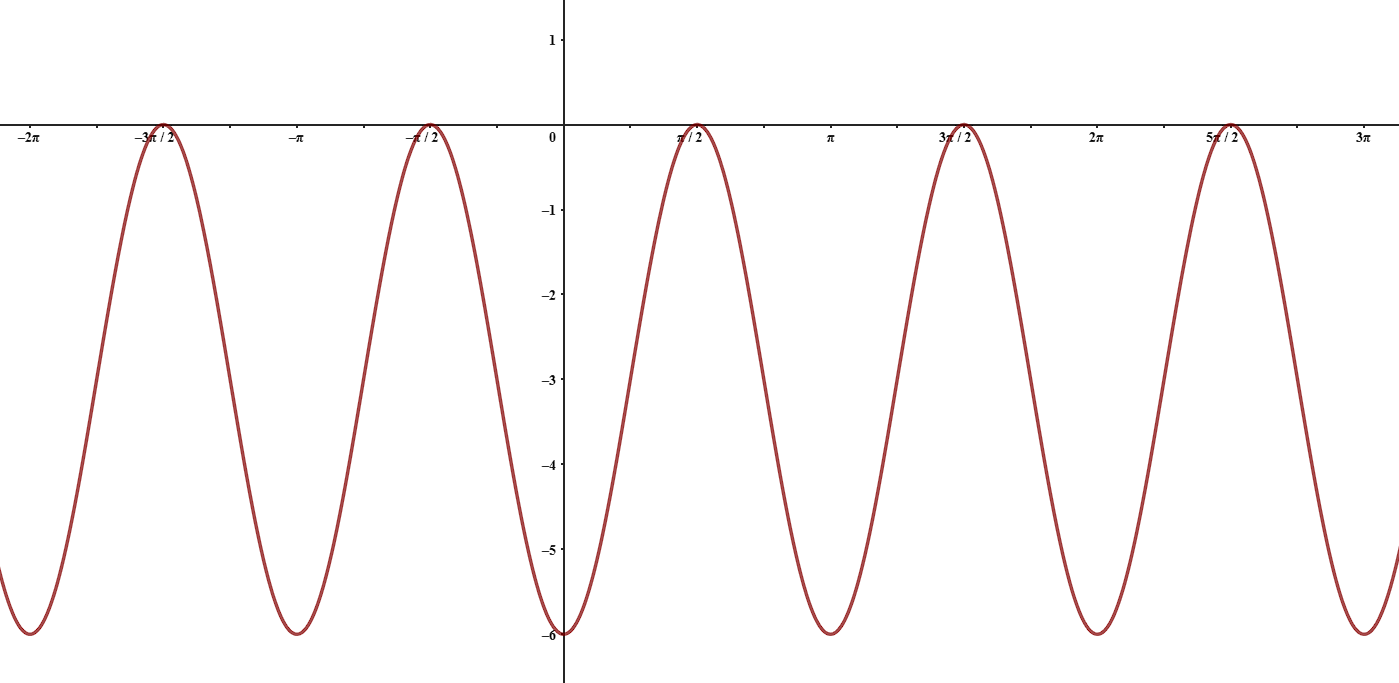
\includegraphics[scale=0.3]{Slike in skice/vaje_vaje_vaje_sinus.png}
    %             \end{figure}
    %         \end{exampleblock}

    %         \note{Avtorica nalog: Darja Turk}

    %     \end{frame}

    %     \begin{frame}
    %         \only<1->{\begin{exampleblock}{Naloga 5}
    %             Brez uporabe računala natančno izračunaj. Zapiši vmesne izračune.
    %             \begin{enumerate}[a]
    %                 \item $\displaystyle \sin\frac{23\pi}{6}$
    %                 \item $\displaystyle \cos\left(-1590^\circ\right)$
    %             \end{enumerate}
    %         \end{exampleblock}}

    %         \only<2->{\begin{exampleblock}{Naloga 6}
    %             Reši enačbi:
    %             \begin{enumerate}[a]
    %                 \item $\displaystyle \sin{2x}+\sqrt{2}\cos x=0$
    %                 \item $\displaystyle 2\cos^2{3x}-\cos{3x}-1=0$
    %             \end{enumerate}
    %         \end{exampleblock}}

    %         \note{Avtorica nalog: Darja Turk}

    %     \end{frame}


    % \subsection{Naklonski kot premice, kot med dvema premicama}
        
    %     \begin{frame}
    %         \frametitle{Naklonski kot premice, kot med dvema premicama}
    %     \end{frame}

\section{Geometrijski liki}

\begin{frame}
    \sectionpage
\end{frame}

\begin{frame}
    \tableofcontents[currentsection, hideothersubsections]
\end{frame}

    \subsection{Obseg in ploščina}

        \begin{frame}
            \frametitle{Obseg in ploščina}
        \end{frame}

    \subsection{Obseg in ploščina kvadrata in pravokotnika}

        \begin{frame}
            \frametitle{Obseg in ploščina kvadrata in pravokotnika}
        \end{frame}

    \subsection{Obseg in ploščina trikotnika}

        \begin{frame}
            \frametitle{Obseg in ploščina trikotnika}
        \end{frame}

    \subsection{Obseg in ploščina paralelograma}

        \begin{frame}
            \frametitle{Obseg in ploščina paralelograma}
        \end{frame}

    \subsection{Obseg in ploščina trapeza in deltoida}

        \begin{frame}
            \frametitle{Obseg in ploščina trapeza in deltoida}
        \end{frame}

    \subsection{Obseg in ploščina pravilnega večkotnika}

        \begin{frame}
            \frametitle{Obseg in ploščina pravilnega večkotnika}
        \end{frame}

    \subsection{Obseg in ploščina kroga}

        \begin{frame}
            \frametitle{Obseg in ploščina kroga}
        \end{frame}



\section{Geometrijska telesa}

\begin{frame}
    \sectionpage
\end{frame}

\begin{frame}
    \tableofcontents[currentsection, hideothersubsections]
\end{frame}

    \subsection{Površina in prostornina}

        \begin{frame}
            \frametitle{Površina in prostornina}
        \end{frame}

    \subsection{Pokončna prizma}

        \begin{frame}
            \frametitle{Pokončna prizma}
        \end{frame}

    \subsection{Pokončni valj}

        \begin{frame}
            \frametitle{Pokončni valj}
        \end{frame}

    \subsection{Pokončna piramida}

        \begin{frame}
            \frametitle{Pokončna piramida}
        \end{frame}

    \subsection{Pokočni krožni stožec}

        \begin{frame}
            \frametitle{Pokočni krožni stožec}
        \end{frame}

    \subsection{Korgla}

        \begin{frame}
            \frametitle{Krogla}
        \end{frame}

    \subsection{Primerjava pokonnih teles}

        \begin{frame}
            \frametitle{Primerjava pokončnih teles}
        \end{frame}

    \subsection{Poševna telesa}

        \begin{frame}
            \frametitle{Poševna telesa}
        \end{frame}

    \subsection{Prisekana telesa}

        \begin{frame}
            \frametitle{Prisekana telesa}
        \end{frame}

    \subsection{Vrtenine}
        
        \begin{frame}
            \frametitle{Vrtenine}
        \end{frame}

\section{Polinomi in racionalne funkcije}

\begin{frame}
    \sectionpage
\end{frame}

\begin{frame}
    \tableofcontents[currentsection, hideothersubsections]
\end{frame}

    \subsection{Polinomi}

        \begin{frame}
            \frametitle{Polinomi}
        \end{frame}

    \subsection{Računanje s polinomi}

        \begin{frame}
            \frametitle{Računanje s polinomi}
        \end{frame}

    \subsection{Ničle polinoma in Hornerjev algoritem}

        \begin{frame}
            \frametitle{Ničle polinoma in Hornerjev algoritem}
        \end{frame}

    \subsection{Graf polinoma}

        \begin{frame}
            \frametitle{Graf polinoma}
        \end{frame}

    \subsection{Polinomska neenačba}

        \begin{frame}
            \frametitle{Polinomska neenačba}
        \end{frame}

    \subsection{Metoda bisekcije}

        \begin{frame}
            \frametitle{Metoda bisekcije}
        \end{frame}

    \subsection{Racionalna funkcija}

        \begin{frame}
            \frametitle{Racionalna funkcija}
        \end{frame}

    \subsection{Racionalna neenačba}

        \begin{frame}
            \frametitle{Racionalna neenačba}
        \end{frame}

    \subsection{Modeliranje s polinomsko in racionalno funkcijo}

        \begin{frame}
            \frametitle{Modeliranje s polinomsko in racionalno funkcijo}
        \end{frame}



\section{Stožnice}

\begin{frame}
    \sectionpage
\end{frame}

\begin{frame}
    \tableofcontents[currentsection, hideothersubsections]
\end{frame}

    \subsection{Krožnica}

        \begin{frame}
            \frametitle{Krožnica}
        \end{frame}

    \subsection{Elipsa}

        \begin{frame}
            \frametitle{Elipsa}
        \end{frame}

    \subsection{Hiperbola}

        \begin{frame}
            \frametitle{Hiperbola}
        \end{frame}

    \subsection{Parabola}

        \begin{frame}
            \frametitle{Parabola}
        \end{frame}

    \subsection{Krivulje drugega reda}

        \begin{frame}
            \frametitle{Krivulje drugega reda}
        \end{frame}

    \subsection{Iracionalna enačba}

        \begin{frame}
            \frametitle{Iracionalna enačba}
        \end{frame}


\end{document}